% Options for packages loaded elsewhere
\PassOptionsToPackage{unicode}{hyperref}
\PassOptionsToPackage{hyphens}{url}
%
\documentclass[
]{report}
\usepackage{lmodern}
\usepackage{amssymb,amsmath}
\usepackage{ifxetex,ifluatex}
\usepackage[titletoc]{appendix}
\usepackage[nottoc]{tocbibind}
\usepackage{graphicx}
\graphicspath{{./images/}}
\ifnum 0\ifxetex 1\fi\ifluatex 1\fi=0 % if pdftex
  \usepackage[T1]{fontenc}
  \usepackage[utf8]{inputenc}
  \usepackage{textcomp} % provide euro and other symbols
\else % if luatex or xetex
  \usepackage{unicode-math}
  \defaultfontfeatures{Scale=MatchLowercase}
  \defaultfontfeatures[\rmfamily]{Ligatures=TeX,Scale=1}
\fi
% Use upquote if available, for straight quotes in verbatim environments
\IfFileExists{upquote.sty}{\usepackage{upquote}}{}
\IfFileExists{microtype.sty}{% use microtype if available
  \usepackage[]{microtype}
  \UseMicrotypeSet[protrusion]{basicmath} % disable protrusion for tt fonts
}{}
\makeatletter
\@ifundefined{KOMAClassName}{% if non-KOMA class
  \IfFileExists{parskip.sty}{%
    \usepackage{parskip}
  }{% else
    \setlength{\parindent}{0pt}
    \setlength{\parskip}{6pt plus 2pt minus 1pt}}
}{% if KOMA class
  \KOMAoptions{parskip=half}}
\makeatother
\usepackage{xcolor}
\IfFileExists{xurl.sty}{\usepackage{xurl}}{} % add URL line breaks if available
\IfFileExists{bookmark.sty}{\usepackage{bookmark}}{\usepackage{hyperref}}
\hypersetup{
  hidelinks,
  pdfcreator={LaTeX via pandoc}}
\urlstyle{same} % disable monospaced font for URLs
\usepackage{longtable,booktabs}
% Correct order of tables after \paragraph or \subparagraph
\usepackage{etoolbox}
\makeatletter
\patchcmd\longtable{\par}{\if@noskipsec\mbox{}\fi\par}{}{}
\makeatother
% Allow footnotes in longtable head/foot
\IfFileExists{footnotehyper.sty}{\usepackage{footnotehyper}}{\usepackage{footnote}}
\makesavenoteenv{longtable}
\setlength{\emergencystretch}{3em} % prevent overfull lines
\providecommand{\tightlist}{%
  \setlength{\itemsep}{0pt}\setlength{\parskip}{0pt}}

%%% Glossary %%%%%%%%%%%%%%%%%%
\usepackage[toc]{glossaries}
\makeglossaries

\newacronym{fxml}{FXML}{FX Markup Language}
\newacronym{repl}{REPL}{Read Evaluate Print Loop}
\newacronym{gui}{GUI}{Graphical User Interface}

\newglossaryentry{implementation-language}{name={implementation language},description={This is the programming language in which the compiler or interpreter is written. It might be the same as either the source language or the target language \cite{compiler-wikibook}}}
\newglossaryentry{source-language}{name={source language},description={The language accepted as input by a compiler, and translated/compiled into a target language \cite{compiler-wikibook}}}
\newglossaryentry{interpreter}{name={interpreter},description={A computer program which examines a computer program written in some source language and carries out the actions required by that program more or less directly, without translating it into some other language \cite{compiler-wikibook}}}
\newglossaryentry{lexical-analysis}{name={lexical analysis},description={The function of lexical analysis is to scan the source program (a sequence of characters arranged on lines) and convert it to a sequence of valid tokens \cite{compiler-wikibook}}}
\newglossaryentry{syntax-analysis}{name={syntax analysis},description={This is an alternative name for parsing. The function of syntax analysis is to check that the source program is grammatically correct, i.e. that we have a valid sequence of tokens \cite{compiler-wikibook}}}
\newglossaryentry{semantic-analysis}{name={semantic analysis},description={The function of semantic analysis is to check that the source program is meaningful. Note that a program can have a valid meaning and still be incorrect if it doesn't do what was really intended \cite{compiler-wikibook}}}
\newglossaryentry{annotated-parse-tree}{name=annotated parse tree,description={A parse tree that is annotated with additional type information \cite{utexas-website}}}
\newglossaryentry{block-statement}{name=block statement, description={A code block is a group of declarations and statements that operates as a unit, usually with its own level of lexical scope. For instance, a block of code may be used to define a function, a conditional statement, or a loop \cite{computerhope-website}}}
\newglossaryentry{expression}{name=expression, description={A combination of letters, numbers, or symbols used to represent a value \cite{computerhope-website}}}
\newglossaryentry{identifier}{name=identifier, description={Identifier means the same as name. The term identifier is usually used for variable names \cite{computerhope-website}}}
\newglossaryentry{keyword}{name=keyword, description={Many programming languages reserve some identifiers as keywords for use when indicating the structure of a program, e.g. if is often used to indicate some conditional code \cite{compiler-wikibook}}}
\newglossaryentry{lexeme}{name=lexeme, description={A word or basic symbol in a language; e.g., a variable name would be a lexeme for a grammar of a programming language \cite{utexas-website}}}
\newglossaryentry{object-binding}{name=object binding, description={The association of a name with a variable or value \cite{utexas-website}}}
\newglossaryentry{parse-tree}{name=parse tree, description={A data structure that shows how a statement in a language is derived from the context-free grammar of the language \cite{utexas-website}}}
\newglossaryentry{parsing}{name=parsing, description={"The process of reading a source language, determining its structure, and producing intermediate code for it \cite{utexas-website}}}
\newglossaryentry{read-evaluate-print-loop}{name=read evaluate print loop, description={Short for read-eval-print loop, REPL is the interactive top level of a programming language interpreter or command line shell. It offers the user a simple prompt, accepts expressions, evaluates them, and prints the result \cite{computerhope-website}}}
\newglossaryentry{recursive-descent parser}{name=recursive descent parser, description={A method of writing a parser in which a grammar rule is written as a procedure that recognizes that phrase, calling subroutines as needed for sub-phrases and producing a parse tree or other data structure as output \cite{utexas-website}}}
\newglossaryentry{reserved-word}{name={reserved word},description={A word in a programming language that is reserved for use as part of the language and may not be used as an identifier \cite{utexas-website}}}
\newglossaryentry{semantic-information}{name=semantic information, description={The meaning of a statement in a language \cite{utexas-website}}}
\newglossaryentry{statement}{name=statement, description={A statement is a single line of code that is used to perform a specific task \cite{computerhope-website}}}
\newglossaryentry{symbol}{name=symbol, description={Refers to a variable stored within the symbol table}}
\newglossaryentry{symbol-table}{name=symbol table, description={A data structure that associates a name (symbol) with information about the named object \cite{utexas-website}}}
\newglossaryentry{token}{name=token, description={A fundamental symbol as processed by syntax analysis. A token may be an identifier, a reserved keyword, a compound symbol, or a single character \cite{compiler-wikibook}}}
\newglossaryentry{type-checking}{name=type checking, description={Tests performed by the compiler to ensure that types of data involved in an operation are compatible \cite{utexas-website}}}
%%%%%%%%%%%%%%%%%%%%%%%%%%%%%%%

%%% General %%%%%%%%%%%%%%%%%%%
\title{The Onyx Compiler}
\author{Louis Lefevre\\BSc Computer Science}
\date{}
%%%%%%%%%%%%%%%%%%%%%%%%%%%%%%%

\begin{document}
\begin{figure}
	
\includegraphics[scale=0.6]{goldsmiths-logo}
	\centering
	\maketitle
\end{figure}
\thispagestyle{empty}

\chapter*{Abstract}
\pagenumbering{roman}
The Onyx Compiler is a program designed with simplicity in mind,
targeted towards learners and novices in the field of programming.
Modern programming languages are not designed for educational purposes,
and as such it can be an arduous task for beginners to start their
journey when it comes to learning coding for the first time. This
projects seeks to solve this problem by providing a language that
contains only the most basic of functionality, simple syntax, insightful
error messages, and an abundance of easy to understand documentation.
The \gls{implementation-language} of choice was Java, as it allows 
for cross-platform compatibility, whilst also utilising JavaFX for development of the
graphical user interface.

\chapter*{Acknowledgements}
A great deal of time and effort was required during the development of
this project, which was only possible with the support and assistance of
a number of people. I would like to begin by first thanking my
supervisor, Dr Edward Anstead, who provided valuable support and
guidance from the beginning. His experience, knowledge, and expertise
contributed a great deal to the formation of the compiler, and yielded
insight that brought the project to where it is today. I would also like
to acknowledge the support provided by my parents throughout the years,
as it is because of them that I have been given the opportunity to
achieve so much and focus on my education. Finally, a special thank you
goes to my girlfriend Atikah, who always recognised my hard work and
encouraged me to be the best I can be. Without her support and love, I
wouldn't be where I am today.

\setcounter{tocdepth}{2}
\tableofcontents

\listoffigures

\chapter{Introduction}
\pagenumbering{arabic}
This report serves as a deeper explanation into the development of the
Onyx Compiler - a program written from scratch that compiles Onyx \gls{source-language}
code down into Java, and aims to provide insight into the inner workings
of the program and the steps taken throughout its development. Whilst
the more complex aspects of compilers and how they work will be
explained in detail, it is assumed that the reader has a substantial
level of knowledge with computers and in computer science as a whole.
Also, keep in mind that whilst there are different types of language
processors (e.g.~\glspl{interpreter}), the term `compiler' will be used as a
blanket term throughout this report.

\section{Aims \& Objectives}
The primary aim of this project is to develop a compiler and programming
language specifically designed for minimalism and simplicity, targeted
towards beginners who are learning programming for the first time. The
language will contain only the bare minimum amount of features required
to teach basic coding skills, with the objective being to reduce
complexity and encourage a straightforward learning experience. Users
will be capable of understanding syntax quickly and intuitively, while
also being able to diagnose issues independently through the use of
informative, coherent, and insightful error messages. They will also be
provided with detailed documentation that avoids the use of jargon, and
a structure which allows for simple navigation when searching for
relevant information. To complement the compiler, a graphical user
interface will also be provided that allows various tasks to be
performed easily and quickly, improving work efficiency. These points
are discussed in more detail in Chapter 3.

\section{Stakeholders}
Stakeholders include clients and users: the former could be a school or
personal tutoring business, whilst the latter is simply anyone who is
looking to learn programming themselves. The project is aimed at people
of all ages, though young children are specifically accounted for by
reducing the complexity of language used in error messages,
documentation, and syntax. The compiler is designed so that it can be
used either by an organisation or an individual, but either way
independent problem solving is encouraged.

\section{Roadmap}
\textbf{Chapter 1 - Introduction}\\
Introduces the report, explaining the aims of the project and details
its stakeholders.

\textbf{Chapter 2 - Background Study}\\
Discusses other projects in the field, explaining the problem and how
other systems fail to solve it.

\textbf{Chapter 3 - Requirements}\\
Lays out each of the pieces of functionality that will be required for
the project.

\textbf{Chapter 4 - Design}\\
Explains how the compiler will be designed, detailing each of the stages
individually.

\textbf{Chapter 5 - Implementation}\\
Demonstrates the methods performed for implementing the compiler's code
base.

\textbf{Chapter 6 - Testing}\\
Describes testing that took place for validating and verifying the
project.

\textbf{Chapter 7 - Evaluation}\\
Evaluates the project based on the requirements defined in Chapter 3,
assessing how successful their implementation was.

\textbf{Chapter 8 - Conclusion}\\
Appraises the overall system, analysing how well it achieves its aims \&
objectives defined in Chapter 1, and reviewing its place in existing
works in the field that were outlined in Chapter 2.


\chapter{Background Study}
The field of compilers is large and complex, with lots of projects
being developed for various purposes. However, it has become
clear that despite this, there is still a void to potentially be
filled.

\section{The Problem}
The issue is that there is a lack of languages designed purely for
learning, and therefore fail to keep beginners in mind. This is important
as there are a number of problems that present themselves exclusively to
beginners, the main one being the lack of intelligible error messages.
Many languages display a verbose string of jargon and numbers whenever
an error occurs, which while useful to experienced programmers, are
completely incoherent to the uninitiated. An example of this can be
seen in Figure \ref{fig:python-error-example}, which demonstrates a
long stack trace coupled with an un-descriptive error message in Python,
and is a distinct example of where the language has made it significantly
more difficult for a novice user to understand where the program went wrong.
Its also worth noting that its rare for a language to even indicate to
the user how to solve a problem clearly, and instead of telling them how
to solve a problem it merely just states the problem itself, with the
rest being up to the user to figure out.

Though perhaps the greatest issue faced is syntax complexity. Whilst
Python solves this issue for the most part, the majority of other
languages arguably have complex syntax that is completely unintuitive.
They aren't designed to read like plain English, and as such it can be
extremely difficult for newcomers to understand what a program is doing
simply by reading over the source code. Also, due to the scale and power
of modern day compilers, there is myriad of \glspl{keyword} and in-built
functions presented to the user. Whilst useful for developing large
projects, the abundance of tools can be overwhelming for some and result
in an information overload. This can have the effect of deterring people
from learning programming soon after they begin.

There is already a big problem with students quitting learning early, as
according to a study by the University of Pennsylvania, on average only
4\% of students successfully complete online courses they've started
\cite{upenn-report}. It was also found that ``roughly 40 percent of students
planning [to undertake] engineering and science majors end up switching to other
subjects or failing to get any degree'' \cite{nytimes-article}. In both of these
situations students drop out early or before they have even begun,
possibly in part due them finding it too difficult to learn the
content, and the frustration of failing early on can result in many
simply giving up.

\begin{figure}
	\centering
	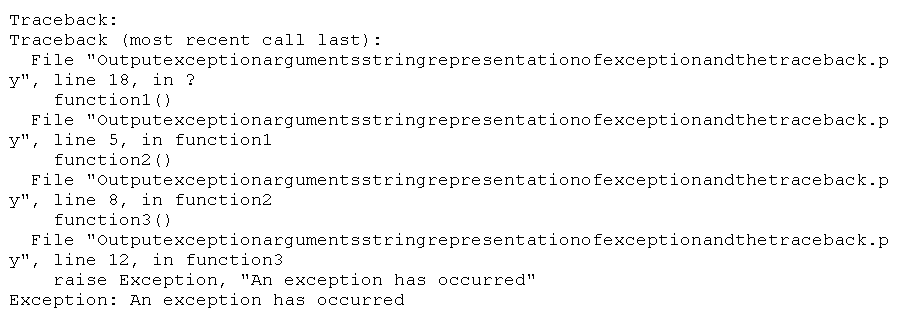
\includegraphics[width=\textwidth]{error-message}
	\caption{Python error message \cite{hackernoon-article}}
	\label{fig:python-error-example}
\end{figure}

\section{Existing Compilers}
There are an abundance of compilers and languages, so it would be
infeasible to go through and review each one. Instead, it would be more
productive to instead focus on languages commonly used by learners.

\subsection{Python}
The most popular language among beginners is Python due to its
flexibility, simple syntax, and abundance of tutorials \cite{simplilearn-article}. In
terms of tackling the problems put forward, it perhaps does the best job
out of the available options. It has intuitive and naturally readable
syntax, an uncommon trait amongst modern languages, whilst also being
rather easy to setup. However, its error messages tend to be verbose,
confusing, and fail to provide a solution. It also contains a large
amount of inbuilt tools and documentation, causing it to appear daunting
at the mere sight of its complexity. Whilst currently being the best
tool for the job, there is vast room for improvement as Python fails to
tackle a large portion of these issues.

\subsection{JavaScript}
JavaScript is another common choice, particularly when it comes to web
development, as a 2019 survey by Stack Overflow found it to be the most
popular language being used by developers \cite{survey-stackoverflow}. It has relatively
flexible and forgiving syntax compared to other object-oriented
languages, whilst also being compatible with all major browsers
\cite{fullstack-article}. However, it can be more difficult to setup and work with due
to the fact its primarily used for front-end web development, which will
also require the use of HTML/CSS. This means that users will also have
to contend with learning those on top of JavaScript and having them work
together, which adds an extra layer of complexity. The error
messages are again wordy and lack explanation, offering no insight for
the inexperienced. It is clear that JavaScript fails to produce
solutions for the presented problems.

\subsection{GitHub Projects}
The GitHub repository known as Awesome Compilers includes a list of 
compilers and \glspl{interpreter} composed by various users \cite{compilers-github}, 
making it useful for reviewing a large selection of projects all at once. 
Based on the descriptions and features lists for the 36 repositories 
included, none were designed to target an audience of beginners nor 
specifically solve the discussed issues.

\chapter{Requirements}
The primary purpose of the Onyx Compiler is to fill the void caused by
the lack of learning-based languages, and is designed solely with
beginners in mind. The compiler is not meant to be complex, and is
instead designed to be as simple as possible in order to teach the
foundations of programming. This project aims to solve each of the
problems previously discussed, with the following detailing the main
goals hoped to be achieved.

\section{Basic Functionality}
The original goal was to keep the language simple with only the bare
minimum number of features, typically those included when teaching introductory
programming courses. A study exploring pedagogical content for
introductory programming courses included a list of topics commonly
taught \cite{pedagogical-report}, and from that, as well as courses and consulting with
tutors, it was found there were five main features to be included:
variables, operators, conditionals, loops, and functions. Given that the
compiler is aimed solely at learners, the amount of functionality
required is not great. The intention is to only focus on the basics, and
so it will only include as much. These are the five main concepts that
Onyx intends to teach its users about, and is essentially the ultimate
goal for users to meet. The purpose of only including the core
components is that it reduces the amount of information users are
presented with, preventing them from feeling overwhelmed.

\section{Data Types, Variables, \& Scope}
The study previously mentioned also found that students often have
difficulty with initializing variables as they ``do not know if it is
necessary to initialize and with what value'', and that students often
had trouble detecting incorrect results due to data type issues
\cite{pedagogical-report}. Scope was also identified as an issue, as students sometimes
failed to realise the difference between variables with identical names
but different scopes \cite{pedagogical-report}. The requirements defined below keep this
in mind, and try to deal with the issues appropriately.

Data types to be included are: integers, doubles, booleans and strings.
The purpose of this selection is provide the common data types which
cover a wide selection of use cases, whilst avoiding the more niche
types that rarely see use and would not typically be used by beginners.
To also avoid unexpected results and remove the need for understanding
type compatibility, only values of the same type can be used together in
\glspl{expression} or an error will be returned.

Originally the goal was to only allow explicit variable declarations,
where the user would have to define the type of a variable during
declaration before it could be used. However, this idea was abandoned as
providing the user with another thing to be concerned with was outside
the boundaries of the projects goal of minimalism. Instead, variables are
implicit and do not need to be declared or given a type, only assigned.
It would be possible for variables to be assigned values of different
data types, regardless of the type the previous value was, though it
would not be possible to use variables containing contradictory data
types with one another.

The compiler also removes a number of features typically found in
languages, such as that of scope. All variables can be accessed
globally, with no such thing as local variables. Whilst this would be an
issue in a more large scale language, the simple nature of Onyx makes
this viable whilst removing the need for the user to learn about scoping
at this level.

\section{Intuitive Syntax}
Syntax will be designed so it reads similarly to regular English, uses
intuitive mathematical \glspl{expression}, and reduces the amount of characters
required for certain \glspl{expression} (e.g.~dynamic typing to remove the need
to declare data types). The objective is to make it at easy as possible
for users to understand what each line is doing just by reading through
the \gls{source-language}. For example, a loop would be written as
\texttt{loop\ myVar\ from\ 0\ to\ 100\ (inclusive)}.

\section{Insightful Error Messages}
One of the greatest pitfalls among novice programmers is their inability
to read and understand error messages, often due to their verbose and
jargon-filled nature, and is one of the biggest difficulties with
students \cite{pedagogical-report}. It is common among popular languages for error
messages to be returned as a long and confusing mess, which while useful
for experienced users, can be devastatingly difficult to decipher for
learners. It is a goal of Onyx to instead provide detailed, easy to read
error messages for the user. Information will be presented in plain
English without the use of jargon, and show where the error occurred
using coloured markings, syntax returns, and line numbers. The simple
yet explanatory error messages are intended to give a clear indication
for where the errors occur, what caused it, and a possible
explanation for how to fix it.

\section{Simple Setup}
An unfortunate truth is that there are a portion of users, particularly
those who are less familiar with computers, who get stuck on the setup and that alone can be
enough to dissuade someone from continuing. That is why Onyx aims to
make setup as easy as possible through the use of its \gls{implementation-language}, Java, 
as the JVM provides the opportunity for cross-compatibility amongst platforms to
remove the need for using a specific operating system. It's even feasible
that it could run on phones, reducing the technological requirement away
from computers. Furthermore, Onyx will be capable of running from an
executable file without any installation, only requiring the user to
download the program to begin.

\chapter{Design}
Designing of the project involved planning in three areas: the layout
and structure of the compiler's source code, the syntax of the language
(also known as the language specification), and the graphical user
interface (\acrshort{gui}).

\section{Compiler Design}
The goal of the compiler is to translate the original Onyx syntax into
Java, which means primarily focusing on front-end compiler construction.
The middle-end and back-end portions are instead handled by Java,
allowing for the development of a language with unique syntax and
functionality without having to worry about the tricky implementation of
close-to-machine-level aspects. A compiler goes through various stages
when processing syntax, with each stage transforming the program
representation in some way. In the form of a pipeline, each component
takes input from its predecessor, transforms it, and feeds the output
forward to the next component \cite{guru99-website}. These stages are
shown in Figure \ref{fig:compiler-phases}.

Throughout the design process, the famous text \emph{Compilers: Principles, Techniques, and Tools} \cite{dragon-book},
also known as the 'Dragon Book', was consulted to help better understand 
the structure of a compiler and the science behind building one.

The top-level package structure can be found in Figure \ref{fig:top-package-diagram}.

\begin{figure}
	\centering
	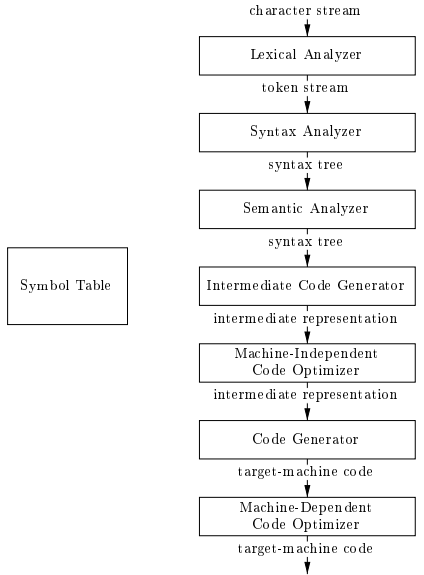
\includegraphics[width=\textwidth]{compiler-phases}
	\caption{Phases of a compiler \cite{dragon-book}}
	\label{fig:compiler-phases}
\end{figure}
\newpage

\subsection{Lexical Analysis}
A compiler will typically always start with \gls{lexical-analysis}, which is
performed by the lexer. It takes the \gls{source-language} as input and scans over
it, typically left to right, and groups the characters into \glspl{lexeme}
\cite{guru99-website}. The lexer represents these \glspl{lexeme} in the form of \glspl{token}
\cite{tutorials-guide}, with each \gls{token} containing information about the type of data
it holds. For example, given the input of an integer, the lexer would
output a \gls{token} that identifies the character's location in the text, its
type (e.g.~an integer \gls{token}), and its value. This process is performed
for all the characters in a given text, and the lexer outputs a stream
of \glspl{token} \cite{kttpro-website}. During this phase, the lexer would also be
responsible for reporting any invalid characters located in the source
code.

The lexer was designed to be capable of handling all types of
characters, whilst also taking into account their context. It had to be
capable of consistently taking in new characters and identifying them
correctly, whilst also adapting to deal with characters found within
particular boundaries. For example, recognising that a number appearing
after open quotations is a part of a string, rather than a \gls{token} in its own
right. The handling of invalid characters must also be considered,
otherwise the lexer would become stuck and be unable to finish.
Having a robust design means never failing to take in characters, and
output valid \glspl{token}.

The package structure for \gls{lexical-analysis} can be found in Figure \ref{fig:lexical-package-diagram}.

In summary, the primary functions of this phase is to:
\begin{itemize}
	\item Take a string of text as input. 
	\item Inspect each individual character, classifying each \gls{token} with its corresponding type, whilst also recognising invalid characters. 
	\item Output a stream of \glspl{token}, often in the form of a list.
	\item Identify invalid characters.
\end{itemize}

\subsubsection{Example}
\begin{verbatim}
	var = 20 + 10
\end{verbatim}
\begin{longtable}[l]{@{}lc@{}}
	\toprule
	Token & Token Type\tabularnewline
	\midrule
	\endhead
	var & Identifier\tabularnewline
	= & Assignment operator\tabularnewline
	20 & Integer\tabularnewline
	+ & Plus operator\tabularnewline
	10 & Integer\tabularnewline
	\bottomrule
\end{longtable}

\subsection{Syntax Analysis}
\begin{figure}
	\centering
	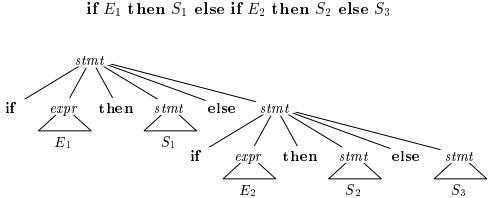
\includegraphics[width=\textwidth]{parse-tree}
	\caption{Parse tree for a conditional statement \cite{dragon-book}}
	\label{fig:parse-tree}
\end{figure}

The second stage of compilation is \gls{syntax-analysis}, also known as
\gls{parsing}, and is performed by the parser. Its role is to take the list of
\glspl{token} produced by the lexer as input, validate the arrangement of
\glspl{token} against the programming languages grammatical rules, and from
that generate a \gls{parse-tree} that represents the structure of the source
program, as shown in Figure \ref{fig:parse-tree}. However, some information
is lost during this process, such as comments and grouping symbols
(e.g. parenthesis) \cite{parsing-tools}. The primary purpose of this component
is to ensure the \glspl{expression} made by the arrangement of \glspl{token}
is syntactically correct, following a format defined by the language being
used \cite{tutorials-guide}. The parser would also identify any syntactical
errors found within the source code.

The parser is designed as a \gls{recursive-descent parser}, which adopts a
top-down \gls{parsing} strategy where it begins at the highest level and works
its way down, building the \gls{parse-tree} as it goes \cite{geeks-website}.
It works with a set of mutually recursive procedures, with one being defined
for each grammatical rule, the parser's structure mirrors the structure of
the grammar \cite{parsing-algorithms}. The input is read from left to right,
taking in \glspl{token} until it reaches the end of the file. Each \gls{token}
would be identified by its type, sending the parser flow in a different direction
depending on the result. The following \glspl{token} would then be checked to
ensure they appear as expected, such as an equals operator \gls{token} appearing
after an \gls{identifier} \gls{token}, and then an \gls{expression} would be returned.
This \gls{expression} would contain all its relevant \glspl{token}, such as in
the case of the previous example: an \gls{identifier}, an equals operator, and
the assignment. In the original design the parser was only able to handle \glspl{expression},
but this was later extended to also process \glspl{statement} so that full programs could be
written all at once since the former only allowed \acrshort{repl}-like behaviour.

\begin{figure}
	\centering
	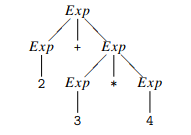
\includegraphics[width=0.5\textwidth]{operator-precedence}
	\caption{Parse tree for the expression 2+3*4 \cite{compiler-design-book}}
	\label{fig:operator-precedence}
\end{figure}

Another aspect that had to be considered was precedence for operators.
It is common for programming languages to use a hierarchy of operator precedences
to decide what will be calculated first in an expression, such as product before
the sum \cite{compiler-design-book}. A parser may define a priority value for
each operator, and during \gls{parsing} they are shuffled around with the parser
being data driven by those priorities, providing an indicator for which \glspl{expression}
to parse next. This makes the inclusion of additional operators much easier, as it
provides the ability to examine operators and see their priority order. An example
of a parse tree produced from the expression \texttt{2+3*4} can be seen in Figure \ref{fig:operator-precedence}.

The package structure for \gls{syntax-analysis} can be found in Figure \ref{fig:syntax-package-diagram}.

In summary, the primary functions of this phase is to:
\begin{itemize}
	\item Retrieve the \glspl{token} from the lexer
	\item Checks if the source code is syntactically correct or not by comparing it against the grammatical rules of the programming language
	\item Construct and output a \gls{parse-tree} representing the syntactic structure of the program
	\item Identify invalid \glspl{expression} and \glspl{statement}
\end{itemize}

\subparagraph{Example}
\begin{verbatim}
	(10 + 20) * 5
	
	    *
	   / \
	  +   5
	 / \  
	10 20
\end{verbatim}

\subsection{Semantic Analysis}
Next comes \gls{semantic-analysis}, which is another stage of \gls{parsing}.
Directly after \gls{syntax-analysis}, \gls{semantic-analysis} takes place as a means
of gathering \gls{semantic-information} about the source code \cite{semantics-wiki}, with
this phase being performed by the type checker in the case of Onyx. It
receives the \gls{parse-tree} from the previous stage and adds extra
information to it, such as: \gls{type-checking} to ensure type conversions are
valid, and \gls{object-binding} for associating variable and function
references with their definitions \cite{compiler-wiki}. This is also where the \gls{symbol}
table is built, adding variables coupled with their values and types. An
\gls{annotated-parse-tree} is output as a result ("annotated" referring to the
extra data having been added to the tree). It is during this phase that
any errors relating to type incompatibility are identified.

Initially, it was designed so that \gls{semantic-analysis} would be performed
within the parser alongside \gls{syntax-analysis}. It was soon found that this
would be implausible since it typically requires a complete \gls{parse-tree}
before being able to add annotations properly, so it was instead moved
to the type checker as an individual component. The type checker
functions by reviewing the type of \gls{expression} or \gls{statement} that is being
executed and comparing the data types of each operand, as well as
reviewing whether the operator being used is compatible. It contains a
series of defined compatibility rules which must be adhered to, the
prevailing rule of which is that only values of the same type can be
used with one another. An error will be returned should there be an
\gls{expression} that fails to meet these rules. Any undeclared variables will
also be identified during this stage, and be returned as errors.

The package structure for \gls{semantic-analysis} can be found in Figure \ref{fig:semantic-package-diagram}.

In summary, the primary functions of this phase is to: 
\begin{itemize}
	\item Get the parse tree from the parser
	\item Validate data type compatibility for operands and operators, ensure variables have been declared, and store variable information within the \gls{symbol-table}
	\item Annotate the \gls{parse-tree} with data type information, producing an \gls{annotated-parse-tree}
	\item Identify mismatched data types, incompatible operands, and undeclared variables
\end{itemize}

\subsubsection{Example}
\begin{verbatim}
a = 30
b = true
c = a * b
\end{verbatim}
This will result in a type-mismatch error as integers and 
booleans are not compatible.

\subsection{Evaluation}
The final stage is the evaluation, performed by the aptly named
evaluator. The purpose of this phase is to calculate the final outputs
of each \gls{statement}, revealing the final result. It reviews the annotated
\gls{parse-tree} and with the extra information gathered by the type checker,
is able to execute each \gls{expression} in Java and return their values. The
output is the final value of the \gls{statement} being evaluated. Its also
worth noting that this is where Onyx diverges when compared to other
compilers, as they often instead follow \gls{semantic-analysis} with
intermediate code generation, code optimisation, and code generator.
However, these stages are instead handled by Java and are not
implemented by Onyx directly, and therefore will not be discussed here.

The design of the evaluator is similar to the parser in regards to the
fact that it works through the tree top-down: searching the tree by
beginning at the closest nodes, working its way down each branch, and
then carrying the result back up the tree as it works through each
\gls{expression}. The result is either used in a larger encompassing
\gls{expression} or stored within a variable, from which the value can be
printed as output. Any \glspl{statement} or \glspl{expression} that fail to store or
use its result in one form or another is discarded.

Also, a unique aspect of this stage is the fact no errors occur here, as
all the necessary error identification should have happened in the prior
stages. However, there are fail-safe exceptions thrown should an error
slip through the cracks, as it helps catch unhandled issues during
development. These are primarily intended to be seen only by developers,
and should not occur in stable versions of the program.

The package structure for evaluation can be found in Figure \ref{fig:generation-package-diagram}.

In summary, the primary functions of this phase is to: 
\begin{itemize}
	\item Obtain the \gls{annotated-parse-tree} from the type checker
	\item Evaluate each \gls{expression} and \gls{statement}
	\item Return the resulting value(s)
	\item Identify any unhandled issues that have gone undetected during the previous stages
\end{itemize}

\subsubsection{Example}
\begin{verbatim}
x = 30
y = 10
x * y
300
\end{verbatim}

\subsection{Symbol Table}
The \gls{symbol-table} is a data structure that is maintained throughout every
phase of a compiler's life-cycle, responsible for storing the names of
\glspl{identifier}, as well as their respective values and data types \cite{tutorials-guide}.
It is also often used for scope management, but this is not present in
Onyx due to the fact it only implements global variables.

The \gls{symbol-table} is designed to be implemented in the form of a hash
map, with the name of the \gls{identifier} as the key and the value and type
as the value. Each of the previous stages have access to the symbol
table, and are able to use it to check whether or not a \gls{symbol} is
contained within the table, as well as retrieve any information about a
particular one. This is most prominent during the type checker and
evaluator, as during these two stages is when types begin to become
relevant for the reasons previously described.

The package structure for symbol management can be found in Figure \ref{fig:symbols-package-diagram},
whilst a working example is displayed in Figure \ref{fig:symbol-table}.

In summary, the primary functions of this component is to: 
\begin{itemize}
	\item Store the names of \glspl{identifier}, along with their value and type
	\item Provide a method for adding and removing \glspl{symbol}
	\item Allow retrieval of information on \glspl{symbol} contained within the \gls{symbol-table}
\end{itemize}

\subsubsection{Example}
\begin{verbatim}
x = 30
y = true

Symbol Table:
x = {
   name: "x",
   value: 5,
   type: integer
}
y = {
   name: "y",
   value: true,
   type: boolean
}
\end{verbatim}

\subsection{Error Handling}
The error handler is responsible for handling errors before continuing
with the compilation process, and like the \gls{symbol-table} is also
accessible to every stage. Throughout each phase, should an error occur,
it is reported to the error handler and then shown to the user in the form
of an appropriately formatted error message. Errors are capable of
occurring in every stage of the compiler apart from the evaluator,
where only exceptions (as seen in Figure \ref{fig:evaluation-exception}) can occur.

In order to prevent interruption, Onyx is designed so that it may
continue compiling should an error occur. While this makes no difference in terms
of the output (as only the error message is returned rather than any
calculated result), it allows certain processes to continue being
performed. For example during the generation of the \gls{parse-tree}, when an
error occurs, the invalid element is replaced by a placeholder (holding a
null value), allowing the \gls{parse-tree} to still be built despite the
invalid syntax. This means the compiler can still provide information
regarding the tree for the rest of the syntax, as well as things like
data types. By not having the compiler quit part way through
compilation, it opens up the possibility of gathering more information, as
well as potentially provide tooling in the future.

The package structure for error handling can be found in Figure \ref{fig:errors-package-diagram}.

In summary, the primary functions of this component is to:
\begin{itemize}
	\item Receive errors from each stage of compilation
	\item Format those errors and generate a detailed message
	\item Output the error message to the user
\end{itemize}

\subsubsection{Example}
\begin{verbatim}
a = true
b = a * 10
Error (2, 2): Binary operator '*' is not defined for type 
'boolean' and 'integer'.
    b = a * 10
\end{verbatim}

\section{Language Specification}
The language specification is what defines a programming language,
detailing what valid syntax is and the behaviour that comes from it.
Onyx was designed with simplicity in mind, so the requirement for
maintaining a simple specification was perhaps the most vital aspect
during design. The main idea was to ensure each piece of functionality
would be written and work as intuitively as possible, in order to leave
little room for the user to be confused as to why something was working
the way it was. The full specification can be found in the Onyx wiki
documentation, found in Appendix \ref{appendix:user-guide}.

\subsection{Data Types}
Onyx was designed to use only the most basic and necessary data types.
Languages such as Java include a large amount of variations for
essentially what is the same data type, except with varying amounts of
memory. For example, integers along with bytes, shorts, and longs. It
was prudent to not consider these redundancies for use, due to the fact
that their benefit of using less memory would not prove useful in the
context of learning. Instead the compiler only contains the following
types: integer, double, boolean, string. This still provides all the
necessary functionality typically found in most languages, except
without the extra level of complexity which may confused new learners.

It is worth noting that the compiler does not allow different data types
to be used together, as seen in Figure \ref{fig:semantic-error}. For example, 
an integer cannot be used with a double in any operations. The purpose of 
this is to help provide a clear distinction between data types and avoid 
unexpected results that are difficult to debug for novices, since type errors 
are not always obvious, particularly when used with variables.

\subsubsection{Example}
\begin{verbatim}
a = 10     # integer
b = 20.0   # double
c = true   # boolean
d = "text" # string
\end{verbatim}

\subsection{Variables}
In the original design it was thought that the language would be
statically typed, requiring all variables to have their data types
declared before use. This was later changed, however, so that the
language was dynamically typed. The reason for this is that it made
things far more simple from a user perspective, as variables could be
reassigned at will without having to be concerned about the declared
type, whilst also avoiding the worry of unexpected results due to the
fact different types are incompatible with one another when operated on.
Not requiring users to declare variables before use was a good method of
simplifying the language even further, since it removed the need to
understand why declaring is necessary.

Variable scope in Onyx is also always kept global, no matter where a
variable is declared. This design choice was primarily made due to the
fact it removed the need for users to learn about scoping, and thus
avoiding issues related to variables being out of bounds. In a much
larger language this would of course be a major issue, but due to the
fact programs written in Onyx will typically be very short in length and
its purpose is simply to learn basic programming functionality, it is not
expected to cause problems.

\subsubsection{Example}
\begin{verbatim}
var = 10   # var is an integer)
var = true # var is now a boolean)
\end{verbatim}

\subsection{Operators}
The compiler specifies use for all the standard mathematical operators
you would typically require to write \glspl{expression}, but also includes some
extra ones such as modulo and power. These two were not going to be
provided initially, but was later added since they could provide
significantly more functionality without being too overbearing for the
user. What was not implemented, however, was the use of increment and
decrement operators. This is mainly due to the difference between
having the unary operators as a prefix and post-fix, which changes the
order in which a value is incremented and returned. Also, it is not as
intuitive for beginners to recognise, unlike other operators, so its use
would likely lead to confusion.

As a slight remedy for the lack of the aforementioned issue, various
assignment operators were specified instead. These would allow variables
to use operators on themselves, providing a shorthand form to prevent
users from being required to write out the full \gls{expression} that includes the
\gls{identifier} name. It was originally unclear whether this would be added
at all since the same operation is still possible with the longhand
form, but it was decided to be intuitive enough to keep in. Figure \ref{fig:loop-statement}
shows an example of an assignment operator being used in a loop.

\subsubsection{Example}
\begin{verbatim}
a = 10
a = a + 15  # longhand form
a += 15     # shorthand form using plus-assignment operator
\end{verbatim}

\subsection{Conditionals}
Conditional \glspl{statement} in Onyx are not too different from traditional
languages and combines attributes from both Python and Java. For
example, the specification doesn't require the use of parentheses for
the condition but still allows them, giving the user the opportunity to
use whichever they feel most comfortable with. However, a more
imperative property is the presence of braces; they are required when
declaring a \gls{block-statement} (code greater than 1 line), but can be
avoided when encompassing only a single \gls{statement}. In the former case
the entire block will be executed, but in the latter only the next
\gls{statement} is executed. It was made a point that Onyx would not feature
\glspl{block-statement} that lack the use of braces, as is allowed in Python.
The reason for this is that it can become very unclear which code
belongs where, particularly when block groupings depend solely on
indentation as in indicator. Whilst this is not an issue when only a
single \gls{statement} is involved, more than that can become confusing for
users and thus has been disallowed entirely.

Another notable design feature is the enforcement of Allman style
indentation, which means open braces must begin on a new line and the
use of single-line conditional \glspl{statement} is disallowed. This is
intended to encourage the use of writing clearer, more modular code,
whilst also providing the additional benefit of having all code written
in Onyx look the same, allowing for easier reviewing of other user's
work.

\subsubsection{Example}
\begin{verbatim}
a = 0

if 1 < 2
    a = 10
else
    a = 20

if a < 20
{
    a = 30
    a *= 5
}
\end{verbatim}

\subsection{Loops}
Loops are designed with intuition in mind, and attempts to adopt
Python's style of looping by having the syntax read more as a sentence.
The purpose is to have loops be clearer in their functionality just by
reading them, unlike in Java where its not easily understandable to the
untrained eye how loops are working without a detailed explanation. Many
of the other properties of loops are the same as conditionals, such as
the enforcement of Allman style indentation and the use of braces in
\glspl{block-statement}, the reasons for which were explained in the previous
section. Though a feature unique to Onyx loops is the inclusion of the
upper bound value, which is uncommon in traditional language
specifications. When looping it is often the case that the final upper
bound value is not executed in the loop's body, which is one of the more
unintuitive aspects of programming. However, the compiler remedies this
by always including the upper value in the execution of the code.

\subsubsection{Example}
\begin{verbatim}
var = 0

loop i from 1 to 10
    var += i
\end{verbatim}

\section{Graphical User Interface}
The \acrshort{gui} was designed with minimalism in mind as it had to be clear how
to use immediately on first use, whilst also not being too daunting for
beginners. The main tools needed for regular use also had to be in clear
sight all the time, with extra functionality being somewhat hidden until
required. Essentially, a sort of abstraction was kept in mind during its
planning.

\subsection{Integrated Development Environment}
The main portion of the \acrshort{gui} would be the IDE, which houses the
components for entering code, running the program, and printing the
output. Aside from a menu, these three things are the only elements
found within the main interface. The purpose of this is to keep it
simple, with only the most necessary components found in plain sight. As
previously mentioned the design will also include a menu bar at the top,
which will be responsible for housing an array of extra functionality.
Some of this extra functionality includes file management (e.g.~opening
and saving files), links for help documentation, and opening the \acrshort{repl}
(discussed in the next section). The IDE also has its own syntax
highlighting, designed with complementary colours in mind that make it
easy to distinguish between syntax and their associated functionality.

The package structure for IDE can be found in Figure \ref{fig:main-package-diagram}.

\subsection{Read Evaluate Print Loop}
An extra feature that comes with the IDE is the \acrshort{repl} - a simple program
that reads input one line at a time and returns a result. It contains a
system for tracking variables, including information about their type,
value, and name. The purpose is to provide a simpler, more visual method
for understanding the basics of writing mathematical \glspl{expression} and
declaring variables. It essentially acts a simplified version of the
compiler and is provided for learners who are struggling to take in
entire programs at once, since instead it gives them the opportunity to
do things one line of code at a time. Its also worth noting that the
\acrshort{repl} doesn't include the use of conditionals or loops, as it is intended
for single-line \glspl{statement} only rather than multi-line ones.

The package structure for REPL can be found in Figure \ref{fig:repl-package-diagram}.

\chapter{Implementation}
The implementation portion of the project involved completing both a
compiler and a \acrshort{gui} individually, the details for which is discussed in
the following sections. It is worth noting that only the primary
components will be discussed and at best in a general sense, as the
codebase is too large and complex to fit into this report. For more
information about the specific workings of each individual method, its
best to refer to the class documentation found in Appendix \ref{appendix:class-docs}.

An image of the final result of the program, consisting of a small code example, can
be found in Figure \ref{fig:ide-overview}.

\section{Compiler Implementation}
Implementation of the compiler meant following the design from the
previous chapter and finding a way to apply it in the \gls{implementation-language}, Java.
It has been built in a way where the components are as modular as possible, with
each stage feeding into the next in the form of a pipeline. This
structure made it rather trivial to isolate each aspect and then
implement the functionality individually, so exploring the source code
isn't too challenging. For assistance in building the foundational classes
and understanding the basics of compiler construction, Immo Landwerth's \emph{Building
a Compiler} video series \cite{compiler-video} was used, as well as the online
book \emph{Crafting Interpreters} \cite{crafting-interpreters}.

The compilers code can be found in Appendix \ref{appendix:compiler-code}, and a brief
explanation of the core functionality in Appendix \ref{Appendix:implementation-video}.

\subsection{Lexer}
The lexer loops through the source text and analyses each character
individually, with the goal of producing a \gls{token} to represent it. The
character is checked to see if it is a line break, white space, digit,
letter, or operator \gls{symbol}, with the first one that matches calling its
corresponding method, which deconstructs the character to discover more
information. In the case of a \gls{reserved-word}, such as 'if' or 'loop',
they are identified as a \gls{keyword} and cannot be used as an \gls{identifier}.
A \gls{token} object is produced that contains data regarding its
type, syntax, value, and position in the text. The \gls{token} is then placed
in the \glspl{token} list, and the next character is reviewed in the same
manner. If a character fails to fall into any of the defined categories
it is deemed invalid and a error is returned, with a `bad \gls{token}' being
produced in its place. The purpose of this filler \gls{token} is to prevent
issues with \gls{parsing} in future stages, as the compiler is designed to be
capable of continuing execution despite mistakes in the code. The final
output of the lexer is a list of \gls{token} objects. For a full list of token types,
view the 'TokenType' package found in Figure \ref{fig:types-package-diagram}.

\subsection{Parser}
The parser retrieves the list of \glspl{token} produced by the lexer and scans
over them, identifying the structure they form to see if it is valid.
Parser execution changes depending on whether the compiler is in \acrshort{repl}
mode, which allows \glspl{expression} to be written as \glspl{statement}, but disallows
the use of loops and conditionals. If \acrshort{repl} mode is not activated, then
the opposite occurs. In the case of the latter, each line is parsed
individually by using line breaks; the presence of a break indicates
that the end of the line has been reached. When a line is parsed it is
first checked to see if it begins with any particular \glspl{keyword} that can
only be found at the start of a line, such as `if', `loop', open braces,
and \glspl{identifier} (those at the start of a line are unique as they act as
the programs print functionality, so when a line begins with solely an
\glspl{identifier} name, its value is printed). Should there be a match the
corresponding method will be called, otherwise the line is deemed an
invalid \gls{statement} and an error is returned.

If the \gls{statement} is valid however, its \glspl{expression} are parsed
recursively by looking at each \gls{token} and matching it with what is
expected. For example, if a \gls{statement} begins with an \gls{identifier} \gls{token},
it looks at the next \gls{token} to see if it is an assignment operator. If
true then it is deemed the code must be assigning a value to a variable,
and an object is produced that contains all the information about that
\gls{statement}. If false, then it continues to check for valid syntax
combinations, such as a binary \gls{expression} where the code is performing a
mathematical operation on the \gls{identifier}. The parser works its way down
the series of possibilities, attempting to find a valid match for the
syntax. If no match is found in the end then the \gls{statement} must contain
invalid syntax and an error is reported, with a dummy \gls{expression} being
produced in its place to allow \gls{parsing} to continue. This process repeats
for each \gls{statement}, with the final output being a \gls{parse-tree} that
contains all the information detailing how the program is structured.

\subsection{Type Checker}
Using the \gls{parse-tree} from the parser, the purpose of the type checker is
to identify the data types being used and see if their use is valid
(e.g.~ensuring only values of the same type are used together in
\glspl{expression}). Similar to the parser, it recursively scans over the tree
nodes, examining each \gls{statement} individually and then producing an
`annotated' \gls{statement} to hold all the information about it. When a
\gls{statement} is parsed the first check is to see what type of \gls{statement} it
is: source (holds the entire program code), \gls{expression} (a single basic
\gls{expression}), block (a series of multiple \glspl{statement}), conditional
(\glspl{statement} that should only run under a certain condition), and loop
(\glspl{statement} to be run a specific amount of times). If a \gls{statement} is
source or block, a list of their contained \glspl{statement} is retrieved and
the process is repeated for each individual one. The final output is an
\gls{annotated-parse-tree}, which is the same as the original except it
contains extra information about data types and \glspl{symbol}.

In the same of conditionals, loops, and \glspl{expression}, the program flow
begins to move further down and starts analysing specific portions of
the \glspl{statement} (e.g.~the condition \gls{expression} of a conditional
\gls{statement}), determining whether they are of the correct type
(e.g.~conditions must be of type boolean). This includes checking that
values used as left and right operands for binary operators are of the
same type, and the unary operators are being applied to valid types
(e.g.~a not-operator cannot be used on a string).

Furthermore, this is where the \gls{symbol-table} is first consulted. If the
user attempts to access a variable that does not exist, an error is
returned. If they try to assign a value to a variable, then a \gls{symbol}
object is created and added to the \gls{symbol-table}. It is worth noting that
the type checker also validates the types of variables, so the type
checking previously discussed applies here. The only exception to this
is when assigning new values to variables, as the type of a variable can
change freely and the new value does not have to be the same type as the
old value. However, assignment operators that employ binary operators
(e.g.~`+=') do not allow type changing and will return an error should
the user attempt to use incompatible types.

\subsection{Evaluator}
The final stage of compilation is performed by the evaluator, which has
the responsibility of calculating the results for every \gls{expression},
running loops and conditionals according to their conditions, and
assigning values to the previously declared \glspl{symbol}. The \gls{parsing} process
for \glspl{statement} is done the same way as it is in the type checker; by
checking the \glspl{statement} type and evaluating each \gls{expression}
individually. The only difference is that the evaluator only returns
information that the user has printed, and any other values are lost.

When an \gls{expression} is evaluated, there is a filtering process which
determines program flow by reviewing its type; each type has
a method specifically designed for it (e.g.~`evaluateBinaryExpression',
`evaluateUnaryExpression'), which examines the values used within that
\gls{expression}. Depending on the data types of the values, program flow is
then directed to another method designed for a specific type
combination. At this point a final check is made to see what type of
operation is being performed on the values (e.g.~addition,
multiplication), and when there is a match the \gls{expression} is computed
accordingly by Java, with the result being returned. This is also where
\glspl{symbol} are given their values, as the type checker only creates the
\glspl{symbol} with their name and type, but doesn't have enough information to
assign a value.

\section{Graphical User Interface}
The \acrshort{gui} has also been built entirely separate from the compiler, with
the only link between them being the user input and the resulting
output. Whilst technically being implemented in Java, the \acrshort{gui} was made
using JavaFX - a software platform for creating desktop applications.
This was further assisted through the use of the JavaFX tool Scene
Builder that provides a visual layout for designing user interfaces
without the need for coding, instead creating the interface with \acrshort{fxml},
which is a XML format used specifically for designing JavaFX \acrshort{gui}'s.

The original draft of the IDE was developed using solely JavaFX and only
contained a handful of features: a menu bar, code area, and output
terminal. Whilst it worked in regards to its most basic purpose of
running code and producing an output, it was buggy and easy to break
when attempting to manipulate the interface in any way. As a result it
was completely overhauled and rebuilt using Scene Builder, which
provided the opportunity to fill in all the gaps that were originally
missed.

The GUI code can be found in Appendix \ref{appendix:gui-code}. A view of the
main interface can also be seen in Figure \ref{fig:ide-overview}, and the
\acrshort{repl} in Figure \ref{fig:repl-overview}.

\subsection{Visual Layout}
The first stage was to focus on designing the interface itself: figuring
out what functionality would be included, where it would go and how it
would look. This was rather trivial as Scene Builders drag-and-drop
functionality, coupled with \acrshort{fxml}'s simplicity, made it extremely easy to
change things and view the results instantly. During this it was
imperative that the interface was adaptable and wouldn't break when
manipulated, as was the problem with the first draft. Fortunately there
were option menus available built to avoid this where each individual
aspect could be told to adapt its size if needed, allowing the entire
\acrshort{gui} to fit into a given space.

\subsection{Controllers}
Next was implementing the functionality for interactions with the
interface, such as when a button is pressed or code is typed. To manage
this, \acrshort{fxml} uses a `controller' - a class it utilises for initialising and
managing the \acrshort{gui}'s elements. Within this class all the methods to be run
are stored, and are called upon by \acrshort{fxml} when their corresponding
component is interacted with. Once this link is made between the \acrshort{gui} and
the controller, the rest of the implementation is plain Java code (with
the exception of outputting information back to the interface, for which
components have their own functionality to do so).

\subsection{File Manager}
File management is handled by the `FileManager' class, providing methods
for opening and saving files. The main consideration taken here was
exception handling - a lot can go wrong if a user opens an invalid file,
doesn't select a file, or a file changes midway through handling. To
deal with this each method returns an extensive amount of exceptions,
each one's purpose being to identify what went wrong. For example, an
invalid file extension error (IllegalArgumentException) is handled
differently to a file not being selected (NullPointerException). This
extra information gives implementing classes the opportunity to handle
individual errors it in the proper way, and avoid unexpected results if
something goes wrong.

For opening and saving files, most of the heavy lifting is performed by
the `FileChooser' - a JavaFX class that provides a dialogue window for
selecting files and directories. Returned from this is a `File' object
pointing to the user's choice, which is then checked for validation. In
the case of opening a file, it is checked to see if it is null (a result
of not selecting a file), cannot be found (the file has been moved or
deleted since being selected), has incorrect permissions (the user
doesn't have read access to the file), or uses an invalid extension (the
user selected a file type outside of the ones specified). If none of
these are true, the file is read and its contents returned. For saving,
the process is identical except for checking that the user has write
access instead, otherwise the contents of the code area are written to
the file. The 'Save' method is used for quick saving a work in progress
file, but is first checked to make sure that it hasn't changed in any
way (moved, renamed, deleted). If it hasn't the contents are instantly
written, and if not it defaults back to the 'Save As' functionality.

The file manager also keeps a track of the current file being worked on
and its contents using the variables `currentFile' and `originalText',
each of which are updated every time the user reads or writes to a file.
The former is used to validate that a file hasn't changed since its last
modification, and is used by the `saveFile' function to decide whether
to save a file immediately, or force the user to create a new file. The
latter is used to track if the original text (from the last accessed
file) is different from the text currently in the code area through use
of the `checkIfSaved' method, providing the opportunity to alert the
user that they have unsaved work if they attempt to perform certain
actions (e.g.~opening a different file or closing the application).

\chapter{Testing}
To test that Onyx successfully meets the requirements and specifications
originally set, the independent procedures of verification and
validation were used as a means of quality assurance.

\section{Validation}
\emph{``Validation. The assurance that a product, service, or system meets the
needs of the customer and other identified stakeholders. It often
involves acceptance and suitability with external customers. Contrast
with verification.''} \\
- Project Management Body of Knowledge \cite{pmbok-book}

The objective of this procedure is to discover whether or not the
compiler is successfully able to meet the needs and requirements
previously defined, in order to prove itself as a useful product amongst
its stakeholders.

\subsection{User Testing}
At the time of writing, it is currently difficult for user testing to
take place due to the fact the country is currently experiencing a
lockdown due to the ensuing pandemic. As a result, gathering and
contacting people who are available for testing has proved difficult and
resulted in a limited sample. However, despite not being able to test
users directly, it has been possible to get in touch with Nadirah, a
coding tutor who works for the computer training school Spark4Kids and
has experience in helping young children to learn basic programming
skills.

\textbf{Question 1: How do you feel about the scope of the compiler?
Does it have too many or too little features for its intended
purpose?}\\
Nadirah explained that she felt the scope of the compiler was just right;
it covered all the basics without going into too much of the more
complex features, which she often found were confusing for beginners to
deal with. By keeping it limited it made it easier to focus on each
individual aspect and create clearer goals in terms of learning.

\textbf{Question 2: Do you think that the insightful error messages will
be useful for students in helping them figure out problems for
themselves?}\\
She explained that in her experience, students of a young age struggle
to make much sense of error messages and often will simply ask for help
rather than attempt to understand the meaning. This is mostly due to the
verbose and confusing nature of the error messages, but also because
they are younger in age and more unable or unwilling to solve the
problem for themselves. As a result, despite the clearer error messages
they may still not make use of them. However, she did explain that it
would still be useful as it would make it easier for tutors to figure
out the problem themselves and explain it to the student. It was also
noted that older students wouldn't have this issue and would be more
capable of understanding the error messages themselves.

\textbf{Question 3: Do you feel that the compiler would be a useful tool
for students learning programming for the first time?}\\
Due to the well-defined scope of functionality and insightful error
messages, Nadirah agreed that it would prove as a valuable learning tool
for novice programmers. Most modern languages aren't designed for
learning and come with a lot of extra functionality that can be
confusing for beginners to get around, so having a language designed
with learners in mind would make things far easier from a teaching
standpoint.

\textbf{Question 4: Do you think having the syntax being written
completely in English would be easier for students to understand, rather
than using standard mathematical \glspl{expression}?}\\
She came to the conclusion that whilst it would still make sense,
students of a young age wouldn't have any more difficultly understanding
basic maths than they would English, and would only serve to making
writing more verbose. If there was an improvement in code readability,
it would be suppressed by the excess use of characters.

\section{Verification}
\emph{``Verification. The evaluation of whether or not a product, service, or
system complies with a regulation, requirement, specification, or
imposed condition. It is often an internal process. Contrast with
validation.''}\\
- Project Management Body of Knowledge \cite{pmbok-book}

The objective of this procedure is to discover whether or not the
compiler successfully meets the requirements set in terms of
functionality, design and quality, demonstrating that its goals have
been met and it is capable of performing to a high standard. To help
achieve this objective, unit tests have been developed for the major
components of the compilers pipeline, each one using specialised inputs
that help identify errors specific to section being tested. An example of
this can be seen in Figures \ref{fig:test-data-example} and \ref{fig:test-example}.
The following explains the testing that took place, and identifies how it
ensures requirements have been met.

The code used to perform unit testing can be found in Appendix \ref{appendix:unit-test-code}.

\subsection{Lexer Testing}
In the original design of the lexer, its primary requirement was to be
capable of taking a string as input, inspecting each character and
categorising it into a \gls{token} with the corresponding type, and then
outputting a list of \glspl{token}. Since all of the tests assess by default
the input of strings and output of \glspl{token}, the main focus becomes the
categorising of \glspl{token}. This was rather trivial as it simply required
the input of single character or word, and then examining the type of
the single \gls{token} found within the returned list, seeing if it matched
what was expected. This was repeated for every character that was
defined within the language, and the tests passing successfully meant
that they were all being identified correctly.

\subsection{Parser Testing}
The parsers function is to check if the source code is syntactically
correct by comparing it against the grammatical rules of the language.
Given the large amount of possibilities in terms of combinations of
\glspl{token}, the first step was to break down the tests into different
\gls{expression} categories: literal, unary, binary, \gls{identifier}, assignment,
and parenthesised \glspl{expression}. Each one would be responsible for
implementing tests for its assigned \gls{expression} type, making it easy to
discover which \gls{expression} failed and the location the issue occurred in
the parser. The tests would simply run the input through the parser and
examine the type of \gls{expression} that was returned, and check that it
matched against the expected outcome.

In order to expand these test cases they were also used in conjunction
with one another, for example, all the tests were wrapped in parentheses
and then passed as parenthesised \glspl{expression}, allowing the amount of
inputs to expand massively without the need to manually add extra cases.
This was rather vital to include, as otherwise it would have meant
either a lot of boilerplate code or lack of edge case testing. In any
case, the passing of the tests provided clarity in the fact that the
parser would correctly verify the syntactic precision of the source
code.

\subsection{Type Checker Testing}
Validating the type checker was rather similar to the parser in terms of
how it was implemented, as not much changes outside of data types. Again
each test was compartmentalised into various categories, with the result
being compared against the expected \gls{expression} type. Though since the
role of the type checker is to validate type compatibility between
operands and operators, the successful return of the correct \gls{expression}
type meant that type validation was achieved and its function was
performed correctly.

\subsection{Evaluator Testing}
The evaluator's main job is to evaluate each \gls{expression} and \gls{statement},
returning the resulting values. This was particularly simple to test
since it only required surveying the final result. Each unit test would
take \glspl{expression} of a particular type, same as previously, and evaluate
the results by running them through the evaluator. The values returned
were then compared against the expected outcome, and if they matched
then the tests passed. It was again rather imperative that this stage
used a substantial pool of inputs for testing, as the amount of
possibilities is extremely large and would potentially reveal a
significant number of edge case issues.

\subsection{Error Handler Testing}
The final stage of unit testing takes place within the error handler,
whose primary responsibility is to receive errors and output them to the
user. Up until this point the unit tests have focused on correct inputs
rather than incorrect ones, so this is where invalid syntax is purposely
passed to see if the expected error message is returned. This was broken
down into three categories: lexical errors occurring in the lexer,
syntax errors occurring in the parser, and semantic errors occurring in
the type checker. If the broken syntax resulted in the expected error
occurring, it can be verified that the compiler successfully handles
errors should they transpire.

\chapter{Evaluation}
The success of the project is largely based on whether or not the
requirements previously discussed in Chapter 3 have been met, with each
of the primary pieces of functionality from the original plans being
reviewed.

\section{Basic Functionality}
The goal for implementing only the bare minimum amount of features was
successful, with variables, operators, conditionals, and loops being
include. Each of these is kept simple and they are capable of working
together in order to form a functioning compiler. The only missing
component is functions, as they were not prioritised and ended up not
being completed. However, they are not vital in regards to overall
functionality and in some regards could begin to complicate the system
unnecessarily as it may be seen as out of scope. As previously discussed
with users, it was also clarified that they agreed the scope was on
point and avoided being too simple or too complex.

\section{Data Types, Variables, \& Scope}
The four data types originally planned were integers, doubles, booleans
and strings, with each one being added successfully. Whilst none of the
types are compatible, there was a plan during development to allow the
use of doubles and integers together. However, it was deemed that this
would be too inconsistent and raise confusion with users over type
compatibility, whilst also producing unexpected results. The main
limitation is that users can only store integer values up to a maximum
of 2\^{}31-1, though this is unlikely to be a common problem as they
will typically be working with smaller numbers for learning. In any
case, it is possible this will be changed so that integers are
automatically converted to longs whenever a number exceeds the limit
(with this process being hidden from the user).

Variables are implicitly defined, not requiring any kind of type
declaration. Whenever a variable is assigned with a new value of a
different type, this conversion is allowed so long as no other operation
is being performed at the same (e.g.~adding, subtracting, etc.). All
variables are also accessible on the global scope, making it possible to
declare them within loops and conditionals.

\section{Intuitive Syntax}
For the syntax, there was a plan to use English words for nearly
everything in order to make it as intuitive as possible, an example
being \texttt{var\ equals\ 10}. Though from user testing it became
apparent that the main audience this was thought to benefit (young
children) would not find it very helpful, and were perfectly capable of
understanding regular mathematical syntax. As a result the language is
written to use English for variables, conditionals and loops, and
operators for any kind of data manipulation. This was a good middle
ground where any written code is not complex and easy to understand,
whilst also not being too verbose.

\section{Insightful Error Messages}
As seen in figures \ref{fig:lexical-error}, \ref{fig:syntax-error},
and \ref{fig:semantic-error}, error messages have been made
as simple as possible, and include line numbers, coloured markings, description
of the error, and a possible solution. An effort was made to remove use of any
jargon and have the problem explained in a clear manner that keeps beginners in mind;
an attempt to remove confusion and frustration during learning experiences.

\section{Simple Setup}
To satisfy the objectives for having a program compatible with all
operating systems whilst also being easy to run, the project was
developed with Java and built as a JAR artefact using IntelliJ IDEA.
Since Java runs within the JVM, the project only requires Java 11 to be
installed for compatibility, and requires no installation as only the
JAR/EXE file needs to be run. Furthermore, Onyx does not have its own
specific file type for opening files, and instead just uses basic text
files. This was to again improve compatibility (as all operating
systems use text files) and allow users to use a familiar file type
instead of a new one.

\chapter{Conclusion}
With the completion of any project comes its assessment; reviewing how
successful or unsuccessful it was, and discovering how much of the
original goals were achieved. Here will be discussed the overall
evaluation of the project, its future prospects, and self-reflection.

\section{Overall Assessment}
Overall, the project has achieved the majority of its goals. As
discussed in chapter 7, all of the functionality defined in the
requirements has been successfully implemented (with the exception of
functions) and the compiler is capable of fulfilling its purpose as a
learning tool. It is completely stable and doesn't crash at any known
point, with a large unit testing infrastructure in place for maintaining
integrity. The \acrshort{gui} has been completed with all the core features, and
has been fitted with a well designed appearance including colour coding
for syntax and error messages. Users are capable of interfacing with the
file system for opening or saving work, and program execution is very
quick. The compiler is compatible with multiple operating systems, and
is able to run without an installation process.

However as mentioned, functions were not implemented in the final
version of the compiler. The \acrshort{gui} also lacks extra features
features which users may find useful for editing code, and doesn't
include a light theme. There are also some bugs still present for niche
input cases, which would need to be fixed before it could be used by a
large user-base. More testing also needs to take place on alternative
operating systems to verify that everything works on each platform.

Furthermore, based on the background study in chapter 2, the compiler is
successful in solving the initial problem presented; Onyx is a compiler
designed purely for learning and keeps beginners in mind the entire
time, adopting a minimalist attitude and presenting itself as a user
friendly alternative to learners. It fills an unoccupied space when
compared to existing compilers, and enhances the field by focusing on an
aspect none others have.

A video of the final product that demonstrates the compilers features
in full can be seen in Appendix \ref{appendix:demo-video}.

\section{Future Development}
While the majority of features were implemented successfully, not
everything was able to be completed in time. The following discusses
what the future may hold for Onyx.

\subsection{Compiler Correctness}
Improving the compiler correctness, which is a a branch of computer
science that deals with attempting to show that a compiler behaves
according to its language specification \cite{correctness-wiki}, would be the primary
improvement prospect. Given that the project was undertaken alone, it is
difficult to test and fix every possible scenario within the time-frame,
particularly in the case of compilers where testing is rigorous and
thorough. Nonetheless, more unit tests are to be added with a wider
array of cases to be covered, with the intention being to reduce the
number of bugs present within the compilers functionality.

\subsection{GUI Clean-up}
Cleaning up the code base for the \acrshort{gui} portion is also planned for the
future, as currently it is rather messy and improvements can be made to improve readability. 
The reason for this is that it was built without prior knowledge of common
practices or conventions, and its design was built on a trial-and-error basis, 
with little rudimentary knowledge of GUI implementation techniques.
Whilst this isn't much of an issue now considering everything functions
as expected, over time it will become more difficult to implement more
features if the foundations are not well established, likely leading to unexpected
results and deeply hidden bugs. The sooner the issue is dealt with,
the easier it will be to fix. Extending the \acrshort{gui} with extra features is
also a prospect, as currently it only contains the most basic
functionality. Filling in the `Edit' menu would be priority since it is
currently empty, and would include options for searching for text,
replacing text, undo/redo changes, copy/paste, and formatting.

\subsection{Implementing Functions}
Functions were included in the original requirements but never added,
though implementing them in the future may be useful. Whilst it is a
concern that functions may be out of scope for Onyx, this issue could be
avoided if built in such a way that is not too intrusive or complex.
In addition, it is possible that including functions may not be seen by 
future users of Onyx as a necessity, in which case the extra layer of complexity 
may be avoided by users if they wish. However, in-built functions that users could call
would prove useful, and could provide functionality for certain
processes such as type conversion.

\section{Self Evaluation}
If I were to do the project again with the knowledge I now have, I would
have spent more time planning the structure of the program out
beforehand; too much time was wasted changing things around, redoing
functionality, and cleaning up code. If strict and well thought-out
planning for the class structure was done, it could've been avoided and
a lot of time would have been saved. I would also spend more time
researching technologies that could be used to help build the project,
such as Scene Builder. Originally, I was unaware of its existence and
wasted a lot of time trying to build the \acrshort{gui} using raw JavaFX code. If I
spent more time investigating other methods, I would have quickly
discovered alternative methods and sped up development dramatically.

Going into this project I had no knowledge or experience working with
compilers, but was fascinated by their complexity and felt confident in
my ability to learn. I've learned a great deal about compiler
construction and each of the individual components that going into
building them, and have improved my skills in programming greatly
throughout development. I was particularly interested in the aspects of
compiler construction, and discovered much more than I had initially
anticipated. Though what I am most proud of is the level to which I 
completed the project; I'm satisfied that it has met the criteria
and standards I originally set for myself, and that I've been able to
produce a strong piece of software that I'll be able to use as a
demonstration for my talents in the future.

\begin{thebibliography}{24}
	\bibitem{dragon-book} 
	Aho, A.V., Sethi, R. and Ullman, J.D. (2006).
	\textit{Compilers: Principles, Techniques, and Tools (2nd ed)}. 
	Addison-Wesley.
	
	\bibitem{pedagogical-report} 
	Bosse, Y., Redmiles, D. and Gerosa, M. (2019).
	\textit{Pedagogical Content for Professors of Introductory Programming Courses}.
	[online] Association for Computing Machinery. Available at:
	\\\texttt{https://dl.acm.org/doi/10.1145/3304221.3319776}
	
	\bibitem{computerhope-website} 
	ComputerHope (2019).
	\textit{Computer Terms, Dictionary, and Glossary}.
	[online] ComputerHope. Available at:
	\\\texttt{https://www.computerhope.com/jargon.htm}
	
	\bibitem{nytimes-article} 
	Drew, C. (2011).
	\textit{Why Science Majors Change Their Minds}.
	[online] The New York Times. Available at:
	\\\texttt{https://www.kttpro.com/six-phases-of-the-compilation-process/}
	
	\bibitem{hackernoon-article} 
	Wengel, G. (2018).
	\textit{How to Read Programming Error Messages}.
	[online] Hackernoon. Available at:
	\\\texttt{https://hackernoon.com/how-to-read-programming-error-messages-22795982c217}
	
	\bibitem{parsing-tools} 
	Tomassetti, G. (2017).
	\textit{Parsing in Java: Tools and Libraries}.
	[online] Tomassetti. Available at:
	\\\texttt{https://tomassetti.me/parsing-in-java/}
	
	\bibitem{parsing-algorithms} 
	Tomassetti, G. (2017).
	\textit{A Guide to Parsing: Algorithms and Terminology}.
	[online] Tomassetti. Available at:
	\\\texttt{https://tomassetti.me/guide-parsing-algorithms-terminology/}
	
	\bibitem{compiler-video} 
	Landwerth, I. (2018).
	\textit{Building a Compiler}.
	[online] YouTube. Available at:
	\\\texttt{https://www.youtube.com/playlist?list=PLRAdsfhKI4OWNOSfS7EUu5GRAVmze1t2y}
	
	\bibitem{compiler-design-book} 
	Mogensen, T. (2010).
	\textit{Basics of Compiler Design (2nd ed)}.
	Springer.
	
	\bibitem{kttpro-website} 
	Munonye, K. (2017).
	\textit{Six Phases of the Compilation Process}.
	[online] The Tech Pro. Available at:
	\\\texttt{https://www.kttpro.com/six-phases-of-the-compilation-process/}
	
	\bibitem{utexas-website} 
	Novak, G. (2019).
	\textit{Compilers: Vocabulary}.
	[online] University of Texas. Available at:
	\\\texttt{https://www.cs.utexas.edu/users/novak/cs375vocab.html}
	
	\bibitem{crafting-interpreters} 
	Nystrom, R. (2020).
	\textit{Crafting Interpreters}.
	[online] CraftingInterpreters. Available at:
	\\\texttt{http://www.craftinginterpreters.com/contents.html}
	
	\bibitem{geeks-website} 
	Pal, R. (2019).
	\textit{Recursive Descent Parser}.
	[online] GeeksforGeeks. Available at:
	\\\texttt{https://www.geeksforgeeks.org/recursive-descent-parser/}
	
	\bibitem{upenn-report} 
	Perna, L., Ruby, A., Boruch, R., Wang, N., Scull, J., Evans, C. and Ahmad, S. (2013).
	\textit{The Life Cycle of a Million MOOC Users}.
	[online] University of Pennsylvania. Available at:
	\\\texttt{https://www.ahead-penn.org/research-projects/life-cycle-mooc-users}
	
	\bibitem{pmbok-book} 
	Project Management Institute (2008).
	\textit{Project Management Body of Knowledge (4th ed)}.
	Institute of Electrical and Electronics Engineers.
	
	\bibitem{guru99-website} 
	Rungta, K. (2019).
	\textit{Phases of Compilers}.
	[online] Guru99. Available at:
	\\\texttt{https://www.guru99.com/compiler-design-phases-of-compiler.html}
	
	\bibitem{survey-stackoverflow} 
	StackOverflow (2019).
	\textit{Developer Survey Results 2019}.
	[online] StackOverflow. Available at:
	\\\texttt{https://insights.stackoverflow.com/survey/2019}
	
	\bibitem{compilers-github} 
	Sumner, R. (2018).
	\textit{Awesome Compilers}.
	[online] GitHub. Available at:
	\\\texttt{https://github.com/rsumner31/awesome-compilers\#compilers-and-interpreters}
	
	\bibitem{tutorials-guide} 
	TutorialsPoint (2020).
	\textit{Compiler Design - Phases of Compiler}.
	[online] TutorialsPoint. Available at:
	\\\texttt{https://www.tutorialspoint.com/compiler\_design/compiler\_design\_phases\_of\_compiler.htm}
	
	\bibitem{compiler-wikibook} 
	Wikibooks Contributors (2020).
	\textit{Compiler Construction}.
	[online] Wikibooks. Available at:
	\\\texttt{https://en.wikibooks.org/wiki/Compiler\_Construction/Glossary}
	
	\bibitem{semantics-wiki} 
	Wikipedia Contributors (2019).
	\textit{Semantics}.
	[online] Wikipedia. Available at:
	\\\texttt{https://en.wikipedia.org/wiki/Semantic}
	
	\bibitem{compiler-wiki} 
	Wikipedia Contributors (2019).
	\textit{Compiler}.
	[online] Wikipedia. Available at:
	\\\texttt{https://en.wikipedia.org/wiki/Compiler}
	
	\bibitem{correctness-wiki} 
	Wikipedia Contributors (2019).
	\textit{Compiler Correctness}.
	[online] Wikipedia. Available at:
	\\\texttt{https://en.wikipedia.org/wiki/Compiler\_correctness}
	
	\bibitem{simplilearn-article} 
	Veeraraghavan, S. (2020).
	\textit{Best Programming Languages to Learn}.
	[online] Simplilearn. Available at:
	\\\texttt{https://www.simplilearn.com/best-programming-languages-start-learning-today-article}
	
	\bibitem{fullstack-article} 
	Yang, D. (2020).
	\textit{The 9 Best Programming Languages to Learn in 2020}.
	[online] FullStackAcademy. Available at:
	\\\texttt{https://www.fullstackacademy.com/blog/nine-best-programming-languages-to-learn}

\end{thebibliography}

\printglossary

\begin{appendices}
	\chapter{Source Code}
	\section{Compiler Code}
	\label{appendix:compiler-code}
	Contains the source code for the compiler.\\
	\url{https://github.com/louislefevre/onyx-compiler/tree/submission/src/main/java}
	\section{GUI Code}
	\label{appendix:gui-code}
	GUI layout and styling resources, including FXML, CSS, and image files.\\
	\url{https://github.com/louislefevre/onyx-compiler/tree/submission/src/main/resources}
	\section{Unit Test Code}
	\label{appendix:unit-test-code}
	Contains the unit tests used for the compiler.\\
	\url{https://github.com/louislefevre/onyx-compiler/tree/submission/src/test/java}

	\chapter{Documentation}
	\section{Class Docs}
	\label{appendix:class-docs}
	Java class documentation for the compilers packages.\\
	\url{https://louislefevre.github.io/onyx-docs/}
	\section{User Guide}
	\label{appendix:user-guide}
	GitHub wiki guide for users and developers.\\
	\url{https://github.com/louislefevre/onyx-compiler/wiki}
	\section{Weekly Logs}
	\label{appendix:weekly-logs}
	Tumblr blog consisting of weekly logs written throughout development.\\
	\url{https://llefe001.tumblr.com/}
	\section{Proposals}
	\label{appendix:proposals}
	Includes copies of the ideation, specification, and interim reports.\\
	\url{https://github.com/louislefevre/onyx-compiler/tree/submission/docs}
	
	\chapter{Videos}
	\section{Compiler Demo}
	\label{appendix:demo-video}
	Demonstration of the compiler and its features.\\
	\url{https://vimeo.com/427916405}
	\section{Implementation Overview}
	\label{appendix:implementation-video}
	Brief explanation for the inner workings of the Onyx Compiler.\\
	\url{https://vimeo.com/427916734}
	\section{Showcase Presentation}
	\label{appendix:showcase-video}
	Showcase presentation discussing the project.\\
	\url{https://vimeo.com/427915621}
	
	\chapter{Screenshots}
	\begin{figure}
		\centering
		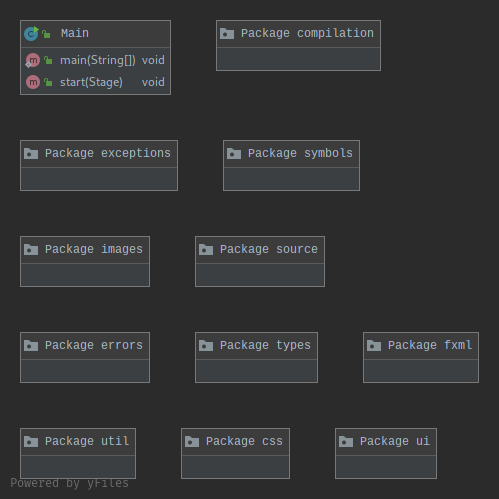
\includegraphics[width=\textwidth]{top-package-diagram}
		\caption{Top-level package}
		\label{fig:top-package-diagram}
	\end{figure}
	\begin{figure}
		\centering
		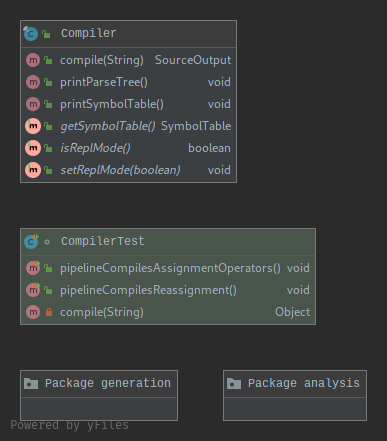
\includegraphics[width=\textwidth]{compilation-package-diagram}
		\caption{Compilation package}
		\label{fig:compilation-package-diagram}
	\end{figure}
	\begin{figure}
		\centering
		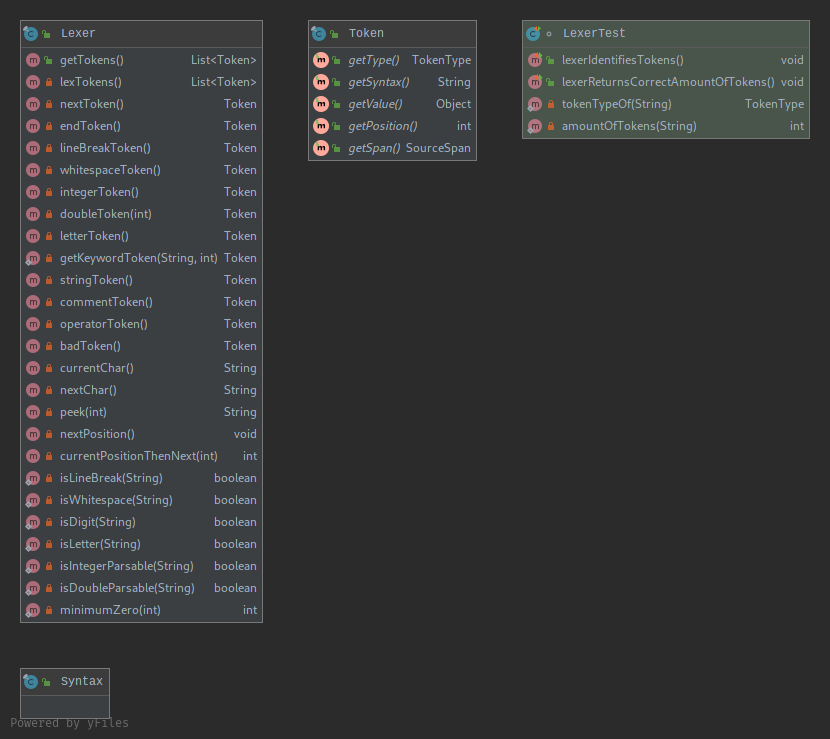
\includegraphics[width=\textwidth]{lexical-package-diagram}
		\caption{Lexical package}
		\label{fig:lexical-package-diagram}
	\end{figure}
	\begin{figure}
		\centering
		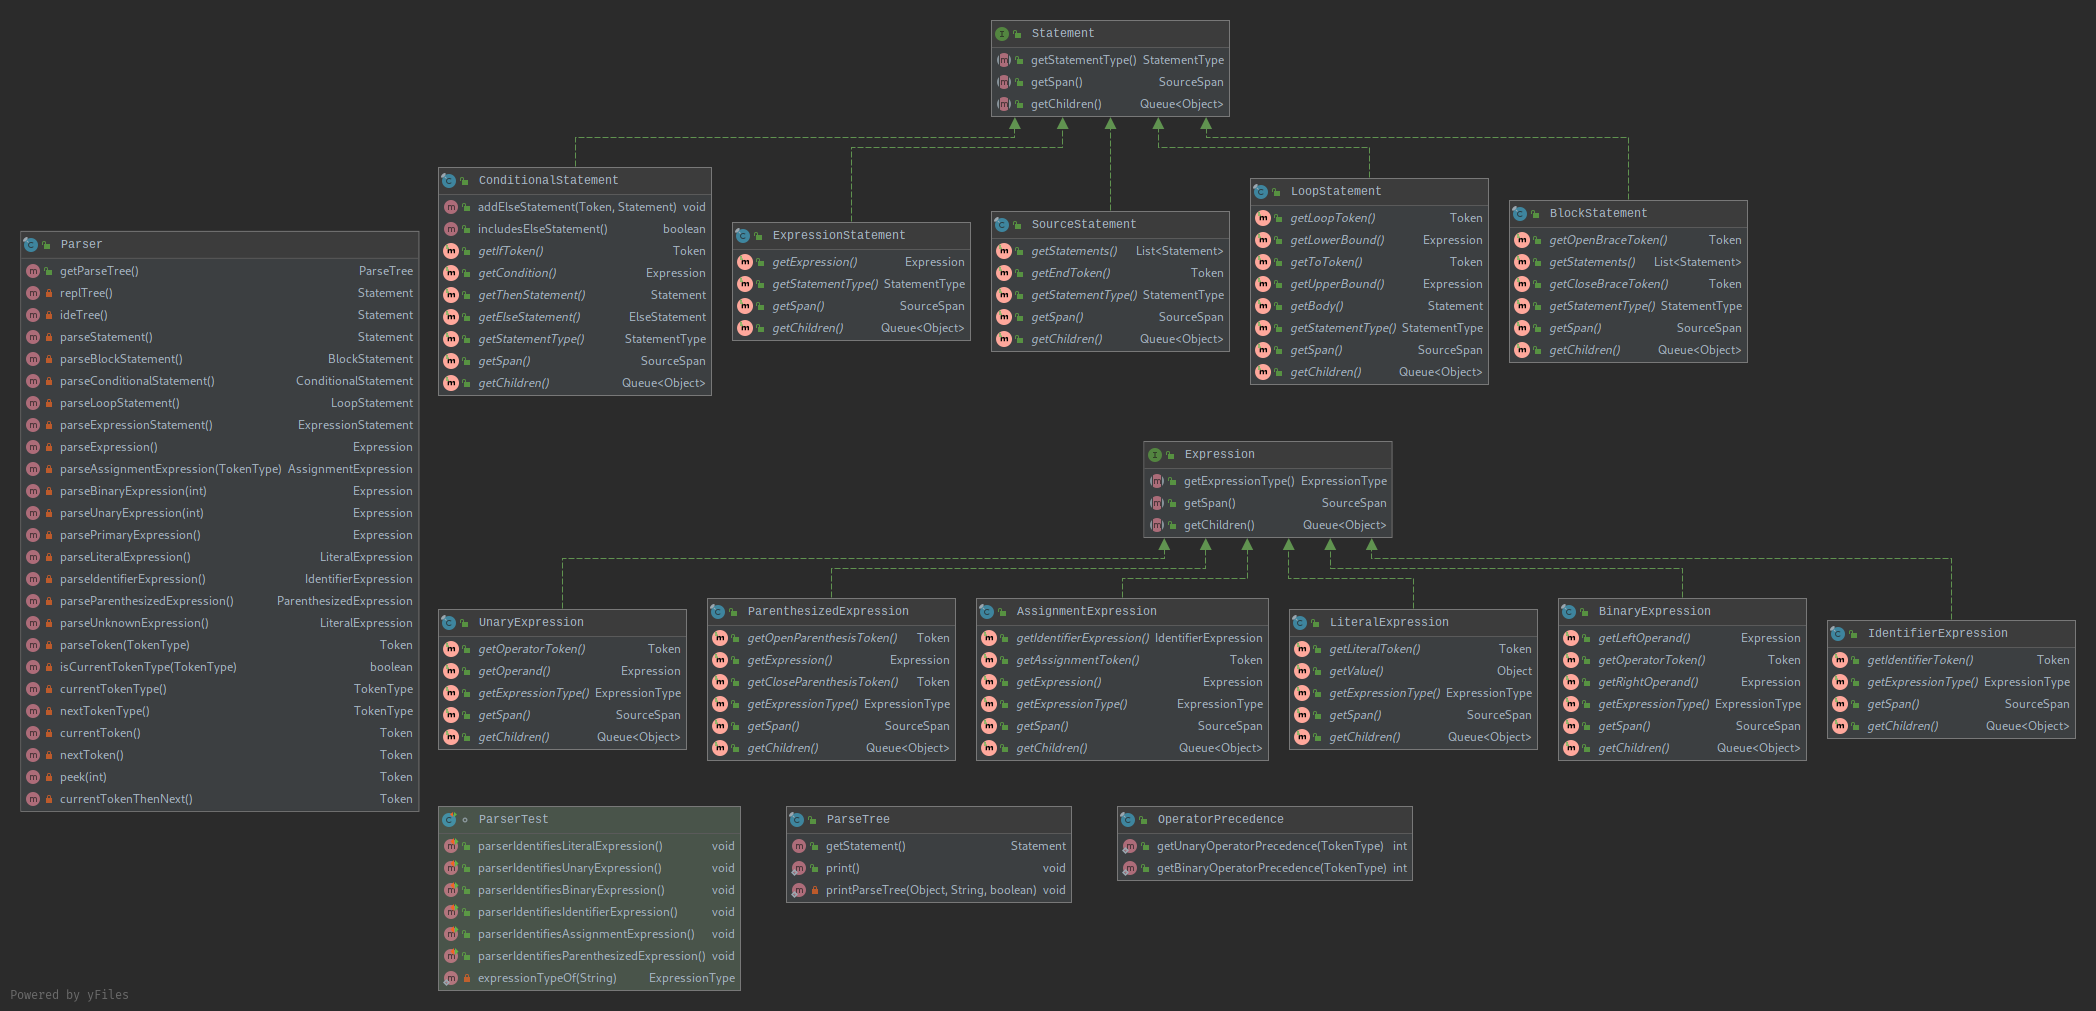
\includegraphics[width=\textwidth]{syntax-package-diagram}
		\caption{Syntax package}
		\label{fig:syntax-package-diagram}
	\end{figure}
	\begin{figure}
		\centering
		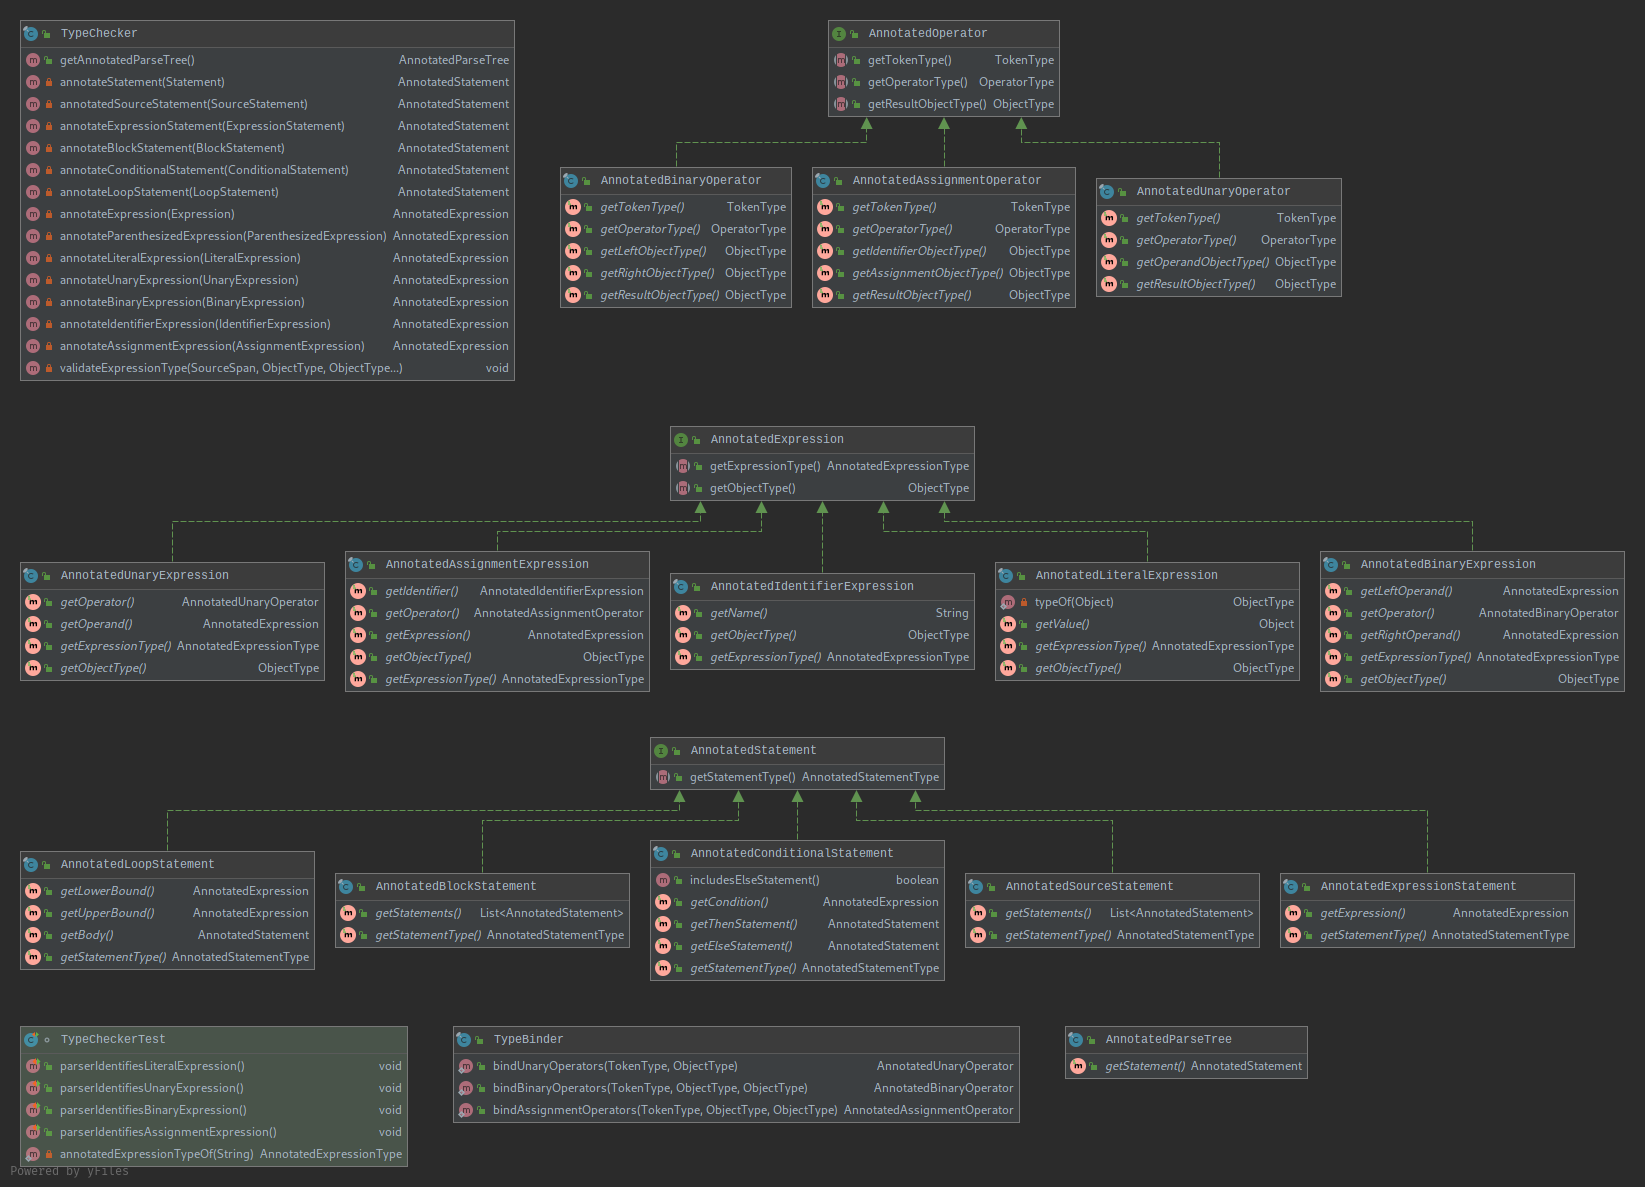
\includegraphics[width=\textwidth]{semantic-package-diagram}
		\caption{Semantic package}
		\label{fig:semantic-package-diagram}
	\end{figure}
	\begin{figure}
		\centering
		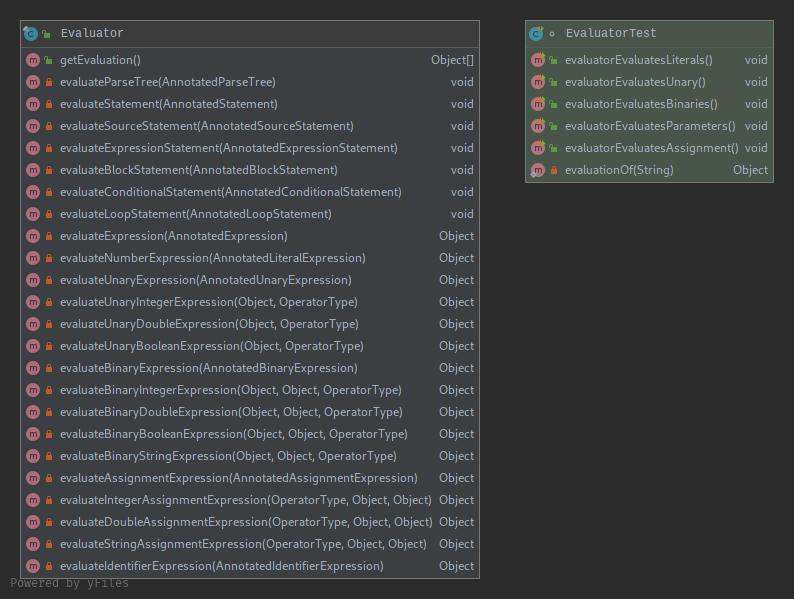
\includegraphics[width=\textwidth]{generation-package-diagram}
		\caption{Generation package}
		\label{fig:generation-package-diagram}
	\end{figure}
	\begin{figure}
		\centering
		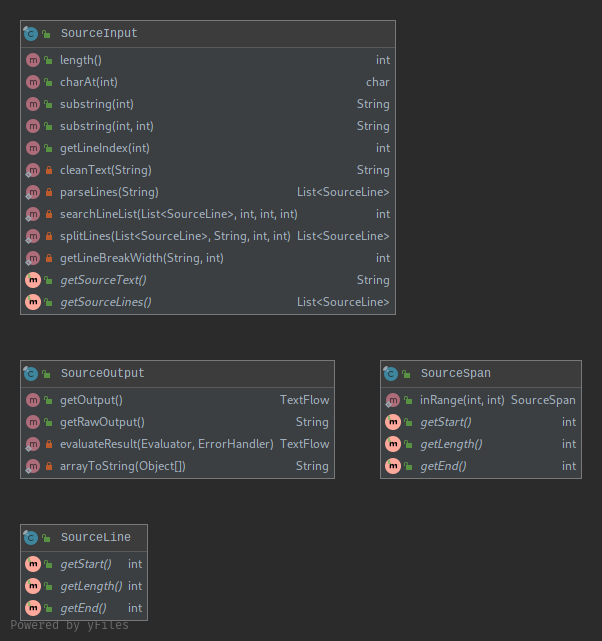
\includegraphics[width=\textwidth]{source-package-diagram}
		\caption{Source package}
		\label{fig:source-package-diagram}
	\end{figure}
	\begin{figure}
		\centering
		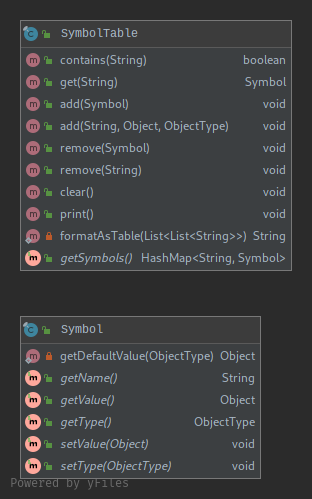
\includegraphics[width=\textwidth]{symbols-package-diagram}
		\caption{Symbols package}
		\label{fig:symbols-package-diagram}
	\end{figure}
	\begin{figure}
		\centering
		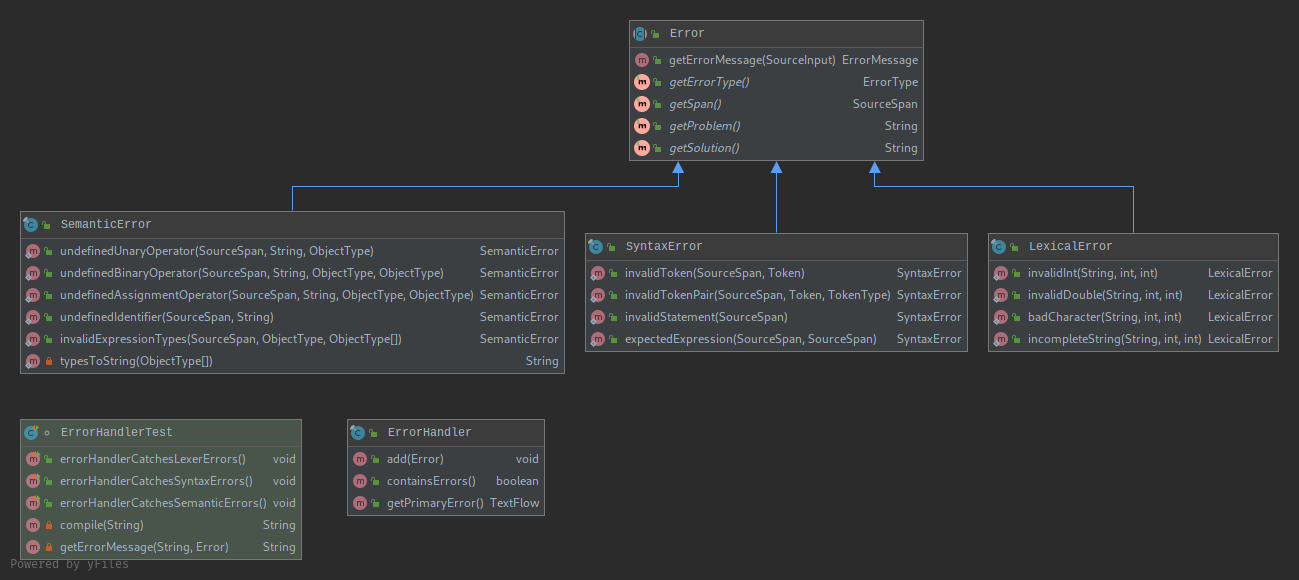
\includegraphics[width=\textwidth]{errors-package-diagram}
		\caption{Errors package}
		\label{fig:errors-package-diagram}
	\end{figure}
	\begin{figure}
		\centering
		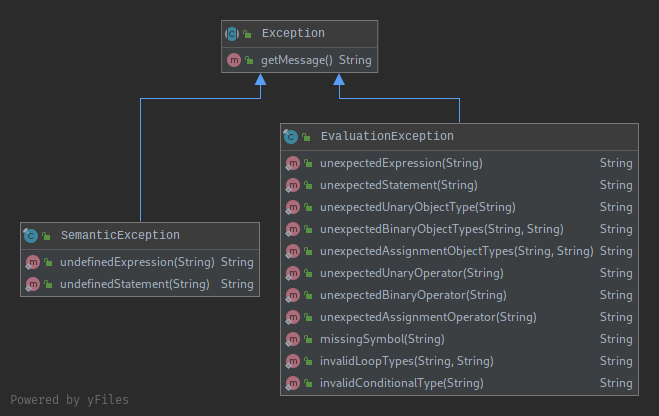
\includegraphics[width=\textwidth]{exceptions-package-diagram}
		\caption{Exceptions package}
		\label{fig:exceptions-package-diagram}
	\end{figure}
	\begin{figure}
		\centering
		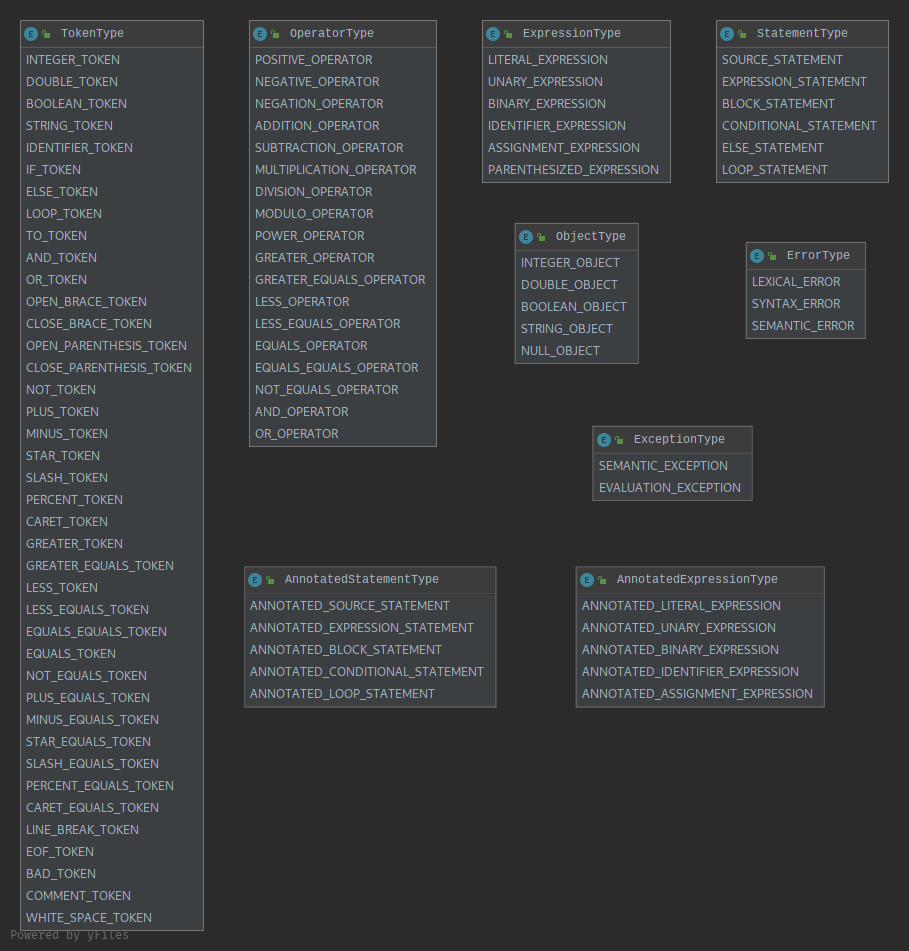
\includegraphics[width=\textwidth]{types-package-diagram}
		\caption{Types package}
		\label{fig:types-package-diagram}
	\end{figure}
	\begin{figure}
		\centering
		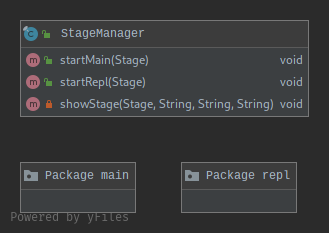
\includegraphics[width=\textwidth]{ui-package-diagram}
		\caption{UI package}
		\label{fig:ui-package-diagram}
	\end{figure}
	\begin{figure}
		\centering
		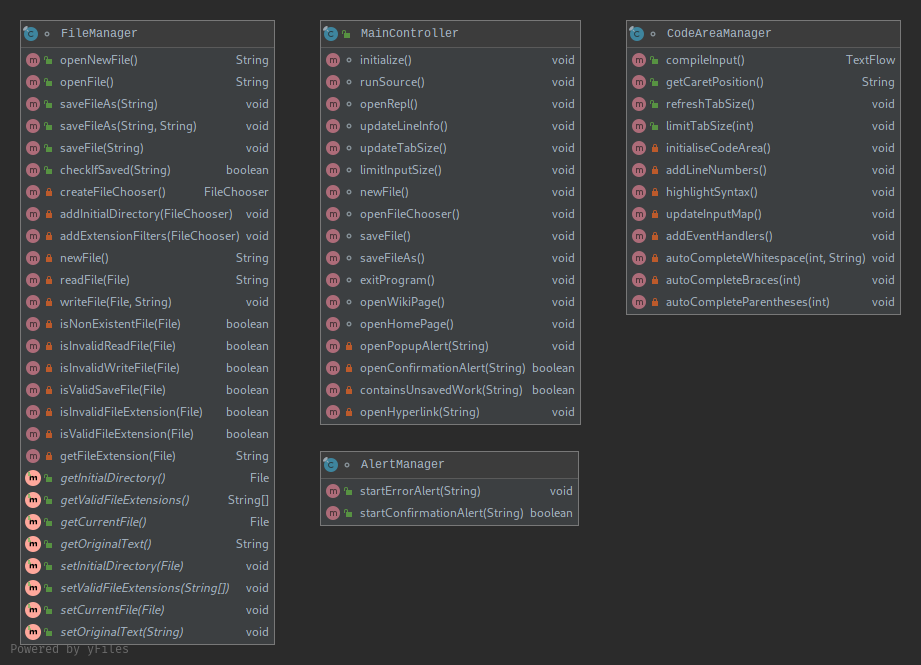
\includegraphics[width=\textwidth]{main-package-diagram}
		\caption{Main package}
		\label{fig:main-package-diagram}
	\end{figure}
	\begin{figure}
		\centering
		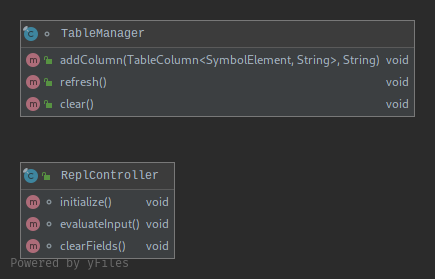
\includegraphics[width=\textwidth]{repl-package-diagram}
		\caption{REPL package}
		\label{fig:repl-package-diagram}
	\end{figure}
	\begin{figure}
		\centering
		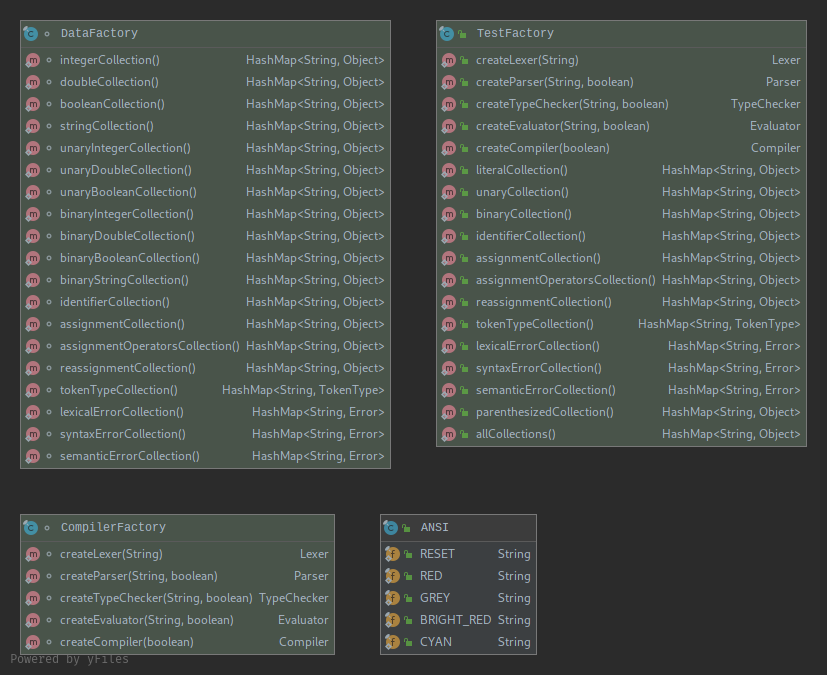
\includegraphics[width=\textwidth]{util-package-diagram}
		\caption{Util package}
		\label{fig:util-package-diagram}
	\end{figure}

	\begin{figure}
		\centering
		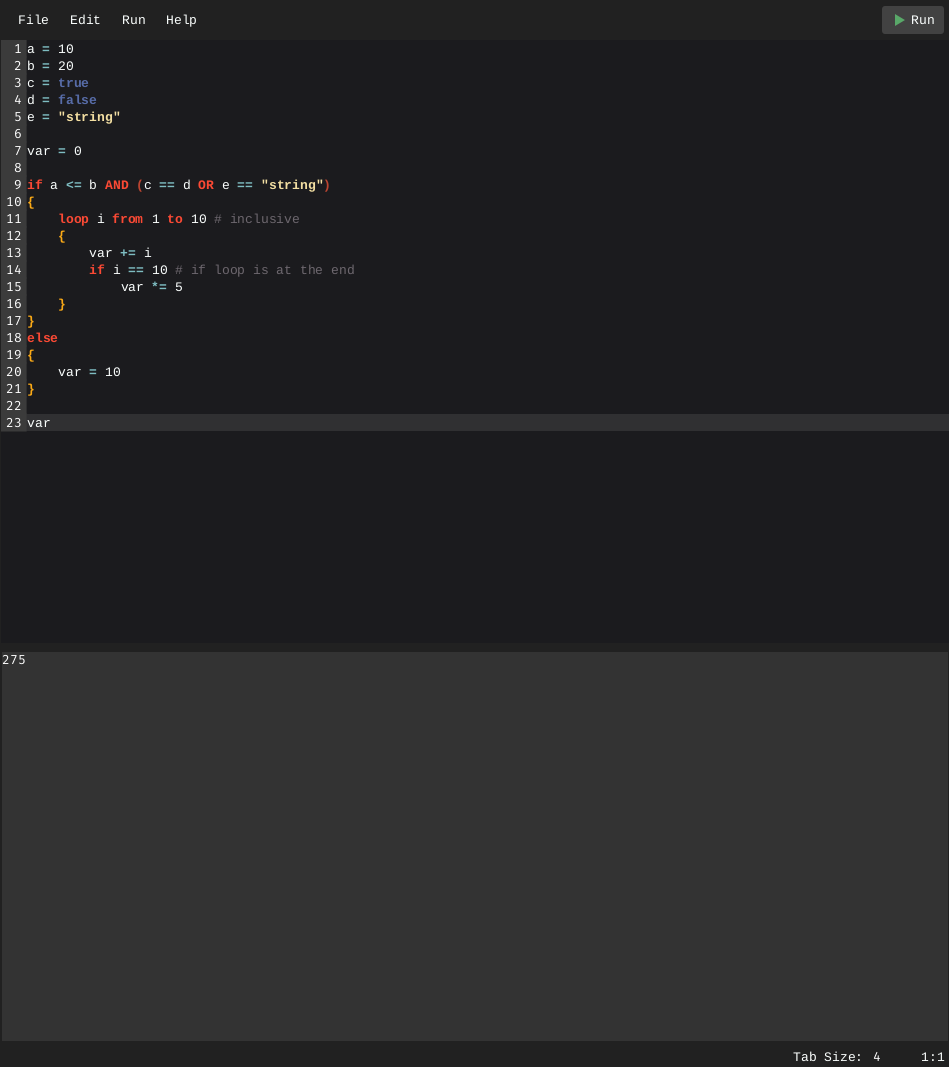
\includegraphics[width=\textwidth]{ide-overview}
		\caption{IDE overview}
		\label{fig:ide-overview}
	\end{figure}
	\begin{figure}
		\centering
		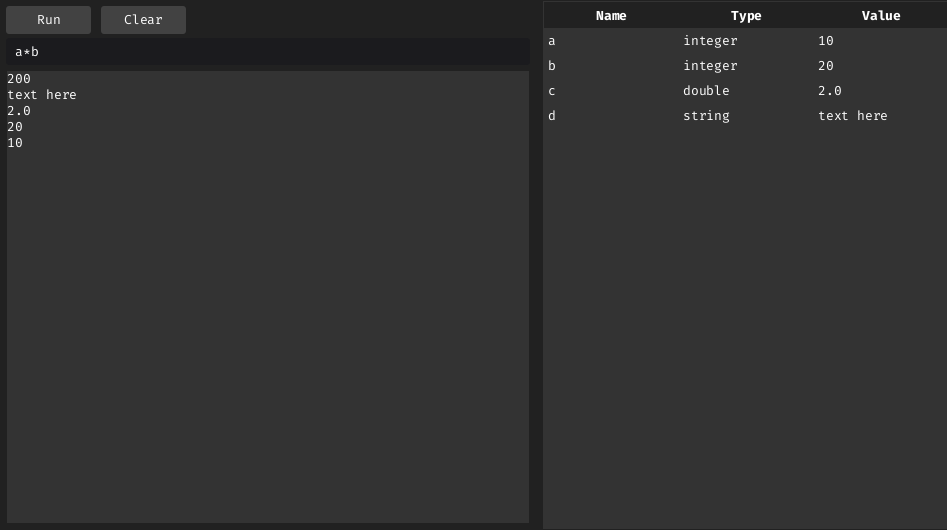
\includegraphics[width=\textwidth]{repl-overview}
		\caption{REPL overview}
		\label{fig:repl-overview}
	\end{figure}

	\begin{figure}
		\centering
		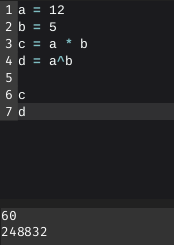
\includegraphics[width=0.45\textwidth]{expression-code}
		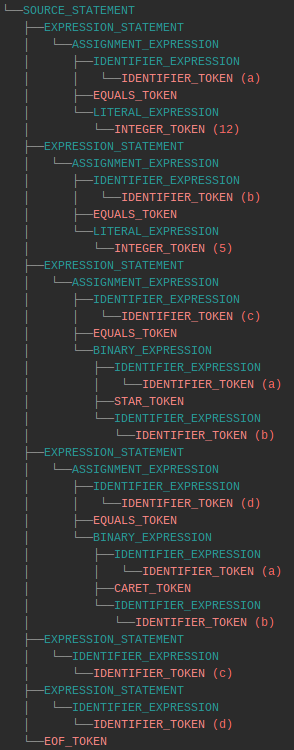
\includegraphics[width=0.45\textwidth]{expression-tree}
		\caption{Expression statement}
		\label{fig:expression-statement}
	\end{figure}
	\begin{figure}
		\centering
		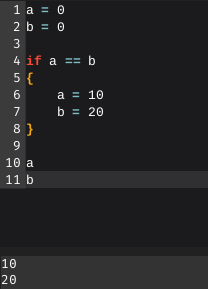
\includegraphics[width=0.45\textwidth]{block-code}
		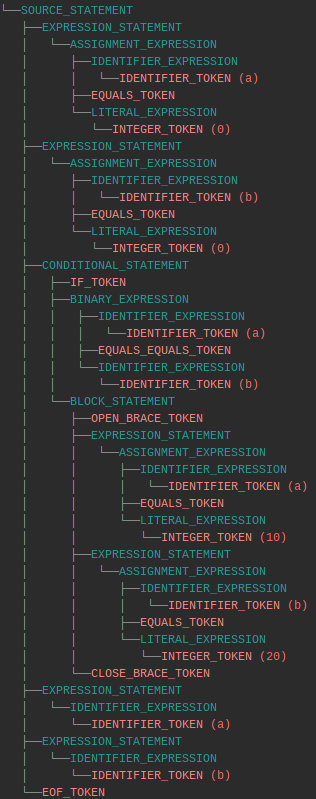
\includegraphics[width=0.45\textwidth]{block-tree}
		\caption{Block statement}
		\label{fig:block-statement}
	\end{figure}
	\begin{figure}
		\centering
		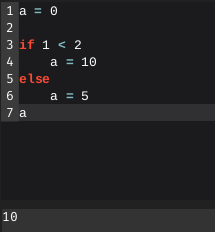
\includegraphics[width=0.45\textwidth]{conditional-code}
		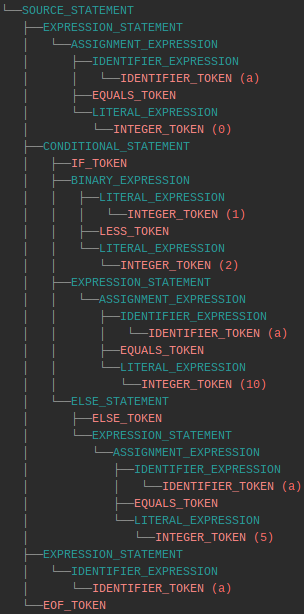
\includegraphics[width=0.45\textwidth]{conditional-tree}
		\caption{Conditional statement}
		\label{fig:conditional-statement}
	\end{figure}
	\begin{figure}
		\centering
		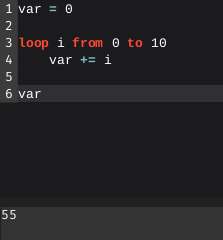
\includegraphics[width=0.45\textwidth]{loop-code}
		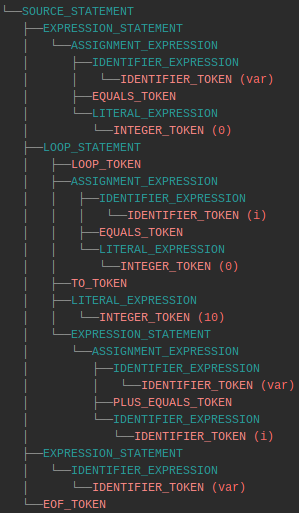
\includegraphics[width=0.45\textwidth]{loop-tree}
		\caption{Loop statement}
		\label{fig:loop-statement}
	\end{figure}
	\begin{figure}
		\centering
		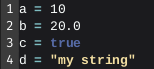
\includegraphics[width=0.45\textwidth]{symbol-table-code}
		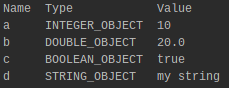
\includegraphics[width=0.45\textwidth]{symbol-table}
		\caption{Symbol table}
		\label{fig:symbol-table}
	\end{figure}
	
	\begin{figure}
		\centering
		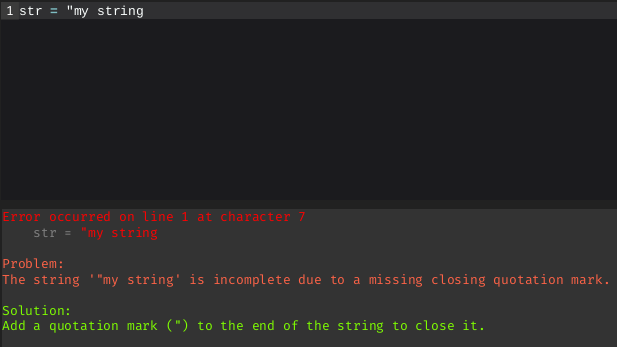
\includegraphics[width=\textwidth]{lexical-error}
		\caption{Lexical error}
		\label{fig:lexical-error}
	\end{figure}
	\begin{figure}
		\centering
		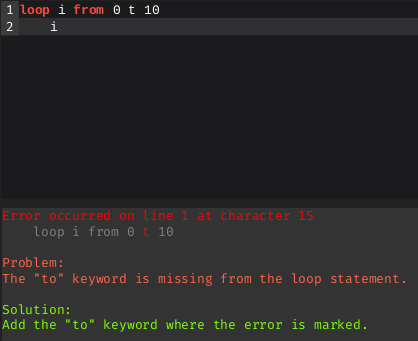
\includegraphics[width=\textwidth]{syntax-error}
		\caption{Syntax error}
		\label{fig:syntax-error}
	\end{figure}
	\begin{figure}
		\centering
		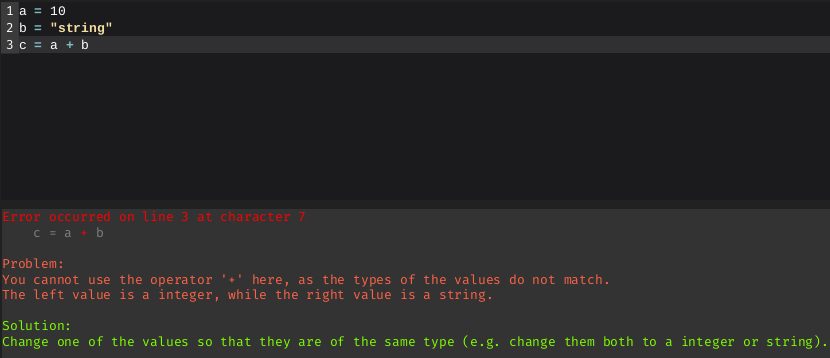
\includegraphics[width=\textwidth]{semantic-error}
		\caption{Semantic error}
		\label{fig:semantic-error}
	\end{figure}
	\begin{figure}
		\centering
		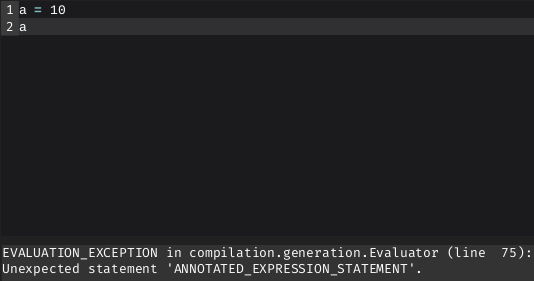
\includegraphics[width=\textwidth]{evaluation-exception}
		\caption{Evaluation exception}
		\label{fig:evaluation-exception}
	\end{figure}
	\begin{figure}
		\centering
		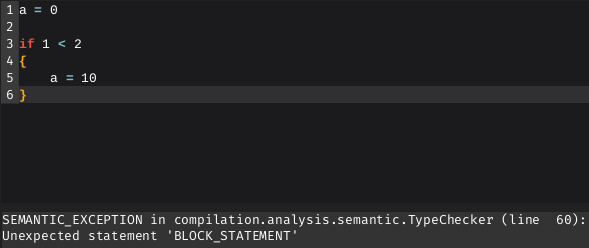
\includegraphics[width=\textwidth]{semantic-exception}
		\caption{Semantic exception}
		\label{fig:semantic-exception}
	\end{figure}
	\begin{figure}
		\centering
		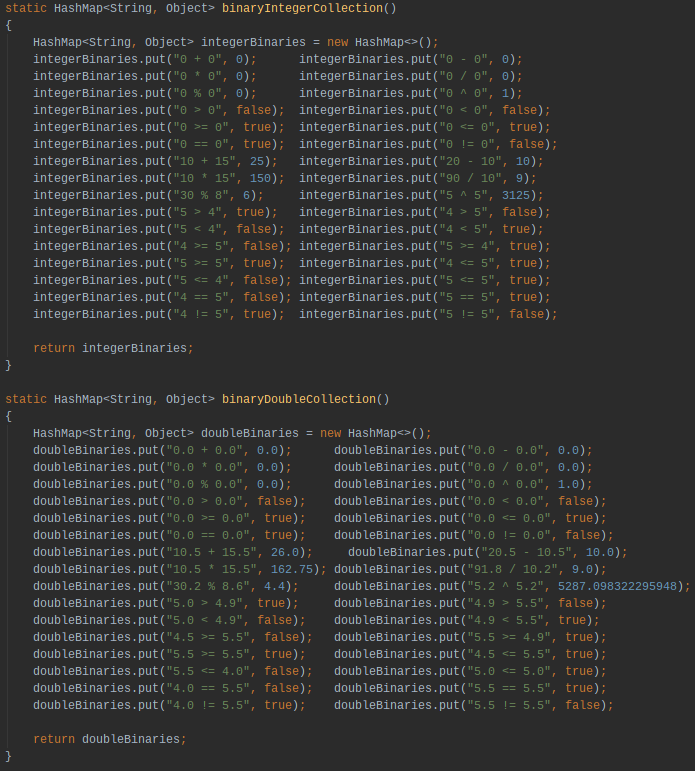
\includegraphics[width=\textwidth]{test-data-example}
		\caption{Unit test data example}
		\label{fig:test-data-example}
	\end{figure}
	\begin{figure}
		\centering
		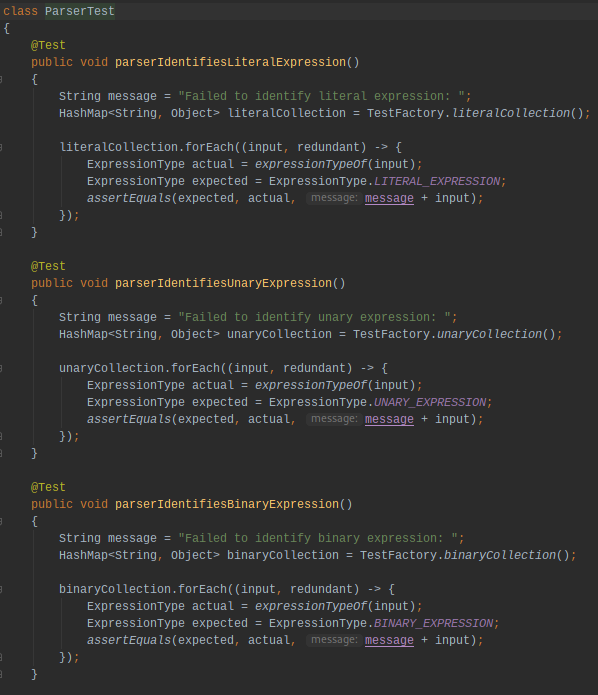
\includegraphics[width=\textwidth]{test-example}
		\caption{Unit test example}
		\label{fig:test-example}
	\end{figure}

\end{appendices}

\end{document}
